% *******************************************************************
% STOP - Bitte zuerst lesen, bevor Sie weitermachen
%
% Einige Dinge müssen Sie an Ihre Bedürfnisse (und die Vorgaben Ihres
% Betreuers anpassen).
%
% 1. Sprache
% Das Template unterstützt Deutsch und Englisch, Standard ist Deutsch.
% Wenn Sie Englisch verwenden wollen, ändern Sie bitte direkt am Anfang
% dieser Datei den Eintrag
%    \newcommand{\hsmasprache}{de}
% auf
%    \newcommand{\hsmasprache}{en}
%
% 2. Zitierstil
% Abhängig von dem gewünschten Zitierstil passen Sie bitte in
% preambel.tex die Einstellungen bei \usepackage[backend=biber...
% an. Wie ist dort genau erklärt.
%
% 3. Doppelseitiger oder einseitiger Druck
% Das Template ist für doppelseitigen Druck eingestellt. Wollen Sie
% einseitig drucken, müssen Sie in preambel.tex die Einstellungen
% für \documentclass ändern. Und zwar von twoside=on auf twoside=off.
%
% 4. Abkürzungen auf richtige Breite einstellen
% In der Datei kapitel/abkuerzungen.tex müssen Sie die _längste_
% Abkürzung in die eckigen Klammern von \begin{acronym} schreiben,
% sonst werden die Abkürzungen nicht richtig ausgerichtet.
% Also z.B. \begin{acronym}[DSGVO].
%
% 5. Unnötige Teile entfernen
% Entfernen Sie die Teile, die Sie nicht brauchen, z.B. Anhänge,
% Quelltextverzeichnis etc. Siehe unten
%
% 6. Silbentrennung
% LaTeX führt eine automatische Silbentrennung durch. Allerdings
% werden Wörter, die bereits einen Bindestrich enthalten nicht
% getrennt, z.B. Datenschutz-Grundverordnung. Wenn Sie Ihren Text auf
% Deutsch schreiben, können Sie dann alternativ "= für den Bindestrich
% im Wort verwenden, z.B. Datenschutz"=Grundverordnung, damit LaTeX
% weiterhin richtig trennt.
% Ist die Silbentrennung aus einem anderen Grund nicht erfolgt, sodass
% das Wort über den rechten Rand hinaussteht oder wenn Sie eine weitere
% Trennstelle wollen, können Sie LaTeX helfen, indem Sie weitere
% Trennstellen angeben. Dies geschieht durch "- als Zeichen, z.B.
% Staats"-vertrag.
%
% 7. Nummerierung der Fußnoten
% LaTeX beginnt die Nummerierung der Fußnoten in jedem Kapitel wieder
% bei 1. Manche Dozenten wollen aber eine durchlaufende Nummerierung
% über die gesamte Arbeit. In diesem Fall gehen Sie in die preambel.tex
% und kommentieren den Befehl \counterwithout{footnote}{chapter} ein.
% *******************************************************************

% Sprache für das Dokument festlegen
\newcommand{\hsmasprache}{de} % de oder en für Deutsch oder Englisch

% Preambel mit Einstellungen importieren
% Dokumententyp und benutzte Pakete
\documentclass[open=right,  % Kapitel darf nur auf rechten Seite beginnen
    paper=a4,               % DIN-A4-Papier
    fontsize=12pt,          % Schriftgöße
    headings=small,         % Kleine Überschriften
    headsepline=true,       % Trennlinie am Kopf der Seite
    footsepline=false,      % Keine Trennlinie am Fuß der Seite
    bibliography=totoc,     % Literaturverzeichnis in das Inhaltsverzeichnis aufnehmen
    twoside=on,             % Doppelseitiger Druck - auf off stellen für einseitig
    DIV=7,                  % Verhältnis der Ränder zum bedruckten Bereich
    chapterprefix=true,     % Kapitel x vor dem Kapitelnamen
    cleardoublepage=plain]{scrbook}

% Pakete einbinden, die benötigt werden
\usepackage{ifthen}               % Logische Bedingungen mit ifthenelse
\usepackage{scrlayer-scrpage}
\usepackage[utf8]{inputenc}       % Dateien in UTF-8 benutzen
\usepackage[T1]{fontenc}          % Zeichenkodierung
\usepackage{graphicx}             % Bilder einbinden

% Setzen von Optionen abhängig von der gewählten Sprache. Die Sprache wird
% in thesis.tex gesetzt.
\ifthenelse{\equal{\hsmasprache}{de}}%
  {%
   \usepackage[main=ngerman, english]{babel}  % Deutsche Sprachunterstützung
   \usepackage[autostyle=true,german=quotes]{csquotes} % Deutsche Anführungszeichen
   \usepackage[pagebackref=false,german]{hyperref} % Hyperlinks
   \newcommand{\hsmasortlocale}{de_DE} % Sortierung der Literatur
  }%
  {%
   \usepackage[main=english, ngerman]{babel} % Englische Sprachunterstützung
   \usepackage[autostyle=true,english=american]{csquotes} % Englische Anführungszeichen
   \usepackage[pagebackref=false,english]{hyperref}  % Hyperlinks
   \newcommand{\hsmasortlocale}{en_US} % Sortierung der Literatur
  }%

\usepackage{xcolor}               % Unterstützung für Farben
\usepackage{amsmath}              % Mathematische Formeln
\usepackage{amsfonts}             % Mathematische Zeichensätze
\usepackage{amssymb}              % Mathematische Symbole
\usepackage{float}                % Fließende Objekte (Tabellen, Grafiken etc.)
\usepackage{booktabs}             % Korrekter Tabellensatz
\usepackage[printonlyused]{acronym}  % Abkürzungsverzeichnis [nur verwendete Abkürzungen]
\usepackage{makeidx}              % Sachregister
\usepackage{listings}             % Quelltexte
\usepackage{listingsutf8}         % Quelltexte in UTF8
\usepackage[hang,font={sf,footnotesize},labelfont={footnotesize,bf}]{caption} % Beschriftungen
\usepackage[scaled]{helvet}       % Schrift Helvetia laden
\usepackage[absolute]{textpos}    % Absolute Textpositionen (für Deckblatt)
\usepackage{calc}                 % Berechnung von Positionen
\usepackage{blindtext}            % Blindtexte
\usepackage[bottom=40mm,left=35mm,right=35mm,top=30mm]{geometry} % Ränder ändern
\usepackage{setspace}             % Abstände korrigieren
\usepackage{scrhack}              % tocbasic Warnung entfernen
\usepackage[all]{hypcap}          % Korrekte Verlinkung von Floats
\usepackage{tabularx}             % Spezielle Tabellen
\usepackage[backend=biber,
  isbn=false,                     % ISBN nicht anzeigen, gleiches geht mit nahezu allen anderen Feldern
  sortlocale=\hsmasortlocale,     % Sortierung der Einträge für Deutsch
                                  %      de_DE: für Deutsch
                                  %      en_US: für Englisch
  autocite=inline,                % regelt Aussehen für \autocite
                                  %      inline: Zitat in Klammern (\parancite)
                                  %      footnote: Zitat in Fußnoten (\footcite)
                                  %      plain: Zitat direkt ohne Klammern (\cite)
  style=ieee,               % Legt den Stil für die Zitate fest
                                  %      ieee: Zitate als Zahlen [1]
                                  %      alphabetic: Zitate als Kürzel und Jahr [Ein05]
                                  %      authoryear: Zitate Author und Jahr [Einstein (1905)]
  hyperref=true,                  % Hyperlinks für Zitate
]{biblatex}                       % Literaturverwaltung mit BibLaTeX
\usepackage{rotating}             % Seiten drehen
\usepackage{harveyballs}          % Harveyballs
\usepackage{chngcntr}

% Kommentieren Sie diese Zeile ein, wenn Sie eine "durchlaufende" Nummerierung bei den
% Fußnoten wünschen, d.h. wenn die Fußnoten nicht bei jedem Kapitel wieder bei 1
% beginnen sollen.
%\counterwithout{footnote}{chapter}

\setlength{\bibitemsep}{1em}      % Abstand zwischen den Literaturangaben
\setlength{\bibhang}{2em}         % Einzug nach jeweils erster Zeile

% Trennung von URLs im Literaturverzeichnis (große Werte [> 10000] verhindern die Trennung)
\defcounter{biburlnumpenalty}{10} % Strafe für Trennung in URL nach Zahl
\defcounter{biburlucpenalty}{500} % Strafe für Trennung in URL nach Großbuchstaben
\defcounter{biburllcpenalty}{500} % Strafe für Trennung in URL nach Kleinbuchstaben

% Farben definieren
\definecolor{linkblue}{RGB}{0, 0, 100}
\definecolor{linkblack}{RGB}{0, 0, 0}
\definecolor{comment}{RGB}{63, 127, 95}
\definecolor{darkgreen}{RGB}{14, 144, 102}
\definecolor{darkblue}{RGB}{0,0,168}
\definecolor{darkred}{RGB}{128,0,0}
\definecolor{javadoccomment}{RGB}{0,0,240}

% Einstellungen für das Hyperlink-Paket
\hypersetup{
    colorlinks=true,      % Farbige links verwenden
%    allcolors=linkblue,
    linktoc=all,          % Links im Inhaltsverzeichnis
    linkcolor=linkblack,  % Querverweise
    citecolor=linkblack,  % Literaturangaben
    filecolor=linkblack,  % Dateilinks
    urlcolor=linkblack    % URLs
}

% Einstellungen für Quelltexte
\lstset{
      xleftmargin=0.2cm,
      basicstyle=\footnotesize\ttfamily,
      keywordstyle=\color{darkgreen},
      identifierstyle=\color{darkblue},
      commentstyle=\color{comment},
      stringstyle=\color{darkred},
      tabsize=2,
      lineskip={2pt},
      columns=flexible,
      inputencoding=utf8,
      captionpos=b,
      breakautoindent=true,
      breakindent=2em,
      breaklines=true,
      breakatwhitespace=false,
      numbers=left,
      numbersep=15pt,
      numberstyle=\tiny\color{black},
      showlines=true,
      numberfirstline=true,
      numbers=none,
      numberstyle=\tiny,
      showspaces=false,      % Keine Leerzeichensymbole
      showtabs=false,        % Keine Tabsymbole
      showstringspaces=false,% Leerzeichen in Strings
      morecomment=[s][\color{javadoccomment}]{/**}{*/},
      literate={Ö}{{\"O}}1 {Ä}{{\"A}}1 {Ü}{{\"U}}1 {ß}{{\ss}}2 {ü}{{\"u}}1 {ä}{{\"a}}1 {ö}{{\"o}}1
}

\urlstyle{same}

% Einstellungen für Überschriften
\renewcommand*{\chapterformat}{%
  \Large\chapapp~\thechapter   % Große Schrift
  \vspace{0.3cm}               % Abstand zum Titel des Kapitels
}

% Abstände für die Überschriften setzen
\renewcommand{\chapterheadstartvskip}{\vspace*{2.6cm}}
\renewcommand{\chapterheadendvskip}{\vspace*{1.5cm}}

\RedeclareSectionCommand[
  beforeskip=-1.8\baselineskip,
  afterskip=0.25\baselineskip]{section}

\RedeclareSectionCommand[
  beforeskip=-1.8\baselineskip,
  afterskip=0.15\baselineskip]{subsection}

\RedeclareSectionCommand[
  beforeskip=-1.8\baselineskip,
  afterskip=0.15\baselineskip]{subsubsection}


% In der Kopfzeile nur die kurze Kapitelbezeichnung (ohne Kapitel davor)
\renewcommand*\chaptermarkformat{\thechapter\autodot\enskip}
\automark[chapter]{chapter}

% Einstellungen für Schriftarten
\setkomafont{pagehead}{\normalfont\sffamily}
\setkomafont{pagenumber}{\normalfont\sffamily}
\setkomafont{paragraph}{\sffamily\bfseries\small}
\setkomafont{subsubsection}{\sffamily\itshape\bfseries\small}
\addtokomafont{footnote}{\footnotesize}
\setkomafont{chapter}{\LARGE\selectfont\bfseries}

% Wichtige Abstände
\setlength{\parskip}{0.2cm}  % 2mm Abstand zwischen zwei Absätzen
\setlength{\parindent}{0mm}  % Absätze nicht einziehen
\clubpenalty = 10000         % Keine "Schusterjungen"
\widowpenalty = 10000        % Keine "Hurenkinder"
\displaywidowpenalty = 10000 % Keine "Hurenkinder"
                             % Siehe: https://de.wikipedia.org/wiki/Hurenkind_und_Schusterjunge

\renewcommand{\footnotesize}{\fontsize{9}{10}\selectfont} % Größe der Fußnoten
\setlength{\footnotesep}{8pt} % Abstand zwischen den Fußnoten

% Index erzeugen
\makeindex

% Einfacher Font-Wechsel über dieses Makro
\newcommand{\changefont}[3]{
\fontfamily{#1} \fontseries{#2} \fontshape{#3} \selectfont}

% Eigenes Makro für Bilder
\newcommand{\bild}[3]{
\begin{figure}[h]
  \centering
  \includegraphics[width=#2]{#1}
  \caption{#3}
  \label{#1}
\end{figure}}

% Wo liegt Sourcecode?
\newcommand{\srcloc}{src/}

% Wo sind die Bilder?
\graphicspath{{bilder/}}

% Makros für typographisch korrekte Abkürzungen
\newcommand{\zb}[0]{z.\,B.}
\newcommand{\dahe}[0]{d.\,h.}
\newcommand{\ua}[0]{u.\,a.}

% Flags für Veröffentlichung und Sperrvermerk
\newboolean{hsmapublizieren}
\newboolean{hsmasperrvermerk}

% Tabellenzellen mit mehreren Zeilen
\newcolumntype{L}{>{\raggedright\arraybackslash}X}
\newcolumntype{b}{l}
\newcolumntype{s}{>{\hsize=.3\hsize}l}

\usepackage{subcaption}
\DeclareCaptionFont{tiny}{\tiny}
\captionsetup{compatibility=false}
\captionsetup{font+=footnotesize}
\captionsetup[sub]{font+=footnotesize}
\captionsetup[table]{belowskip={10pt}}

\DeclareMathOperator*{\argmin}{argmin}

\usepackage{nicefrac}

% Dokumenteninfos importieren
% -------------------------------------------------------
% Daten für die Arbeit
% Wenn hier alles korrekt eingetragen wurde, wird das Titelblatt
% automatisch generiert. D.h. die Datei titelblatt.tex muss nicht mehr
% angepasst werden.

% Titel der Arbeit auf Deutsch
\newcommand{\hsmatitelde}{Untersuchung von Kartierungsalgorithmen unter ROS mit dem Pioneer 3-DX}

% Titel der Arbeit auf Englisch
\newcommand{\hsmatitelen}{Analysis of cartographing algorithms in ROS using the Pioneer 3-DX}

% Weitere Informationen zur Arbeit
\newcommand{\hsmaort}{Mannheim}    % Ort
\newcommand{\hsmaautorvname}{Daniel} % Vorname(n)
\newcommand{\hsmaautornname}{Koch} % Nachname(n)
\newcommand{\hsmadatum}{23.10.2019} % Datum der Abgabe
\newcommand{\hsmajahr}{2019} % Jahr der Abgabe
\newcommand{\hsmafirma}{} % Firma bei der die Arbeit durchgeführt wurde
\newcommand{\hsmabetreuer}{Prof. Dr. Thomas Ihme, Hochschule Mannheim} % Betreuer an der Hochschule
\newcommand{\hsmazweitkorrektor}{} % Betreuer im Unternehmen oder Zweitkorrektor
\newcommand{\hsmafakultaet}{I} % I für Informatik oder E, S, B, D, M, N, W, V
\newcommand{\hsmastudiengang}{IB} % IB IMB UIB IM MTB (weitere siehe titleblatt.tex)

% Zustimmung zur Veröffentlichung
\setboolean{hsmapublizieren}{true}   % Einer Veröffentlichung wird zugestimmt
\setboolean{hsmasperrvermerk}{false} % Die Arbeit hat keinen Sperrvermerk

% -------------------------------------------------------
% Abstract

% Kurze (maximal halbseitige) Beschreibung, worum es in der Arbeit geht auf Deutsch
\newcommand{\hsmaabstractde}{Diese Studienarbeit untersucht Kartierungsalgorithmen wie Google Cartographer, gmapping oder hector\_mapping im Robot Operating System (ROS), einem open-source Meta-Betriebssystem für die Entwicklung von Robotern. Es wird die Funktionsweise der genannten Algorithmen analysiert und ein Package aufgesetzt, welches mit dem Pioneer 3-DX kompatibel ist. Dieses Package wird genutzt, um die Fähigkeit der Algorithmen unter bestimmten Bedingungen in einer 2D-Umgebung zu testen. In diesen Tests schneidet der Google Cartographer auf Grund von genauen Kartierungen und einer Vielzahl an Konfigurationsmöglichkeiten am besten ab.}

% Kurze (maximal halbseitige) Beschreibung, worum es in der Arbeit geht auf Englisch
\newcommand{\hsmaabstracten}{This study evaluates cartographing algorithms like Google Cartographer, gmapping or hector\_mapping within the Robot Operating System (ROS). ROS is an open-source meta operating system for the development of robots. The study analyzes the functionality of these algorithms and sets up a package which is compatible with the Puoneer 3-DX. The package is used then to evaluate the capability of the algorithms in a defined 2D environment. In these tests the Google Cartographer performs best since it creates the most accurate maps and had the most configuration options.}


% Literatur-Datenbank
\addbibresource{literatur.bib}   % BibLaTeX-Datei mit Literaturquellen einbinden

\begin{document}
\frontmatter

% Römische Ziffern für die "Front-Matter"
\setcounter{page}{0}
\changefont{ptm}{m}{n}  % Times New Roman für den Fließtext
\renewcommand{\rmdefault}{ptm}

% Titelblatt
% -------------------------------------------------------
% In dieser Datei sollten eigentlich keine Veränderungen mehr
% notwendig sein. Alle Einstellungen erfolgen in docinfo.tex
% -------------------------------------------------------

\thispagestyle{empty}

% Fakultäten der HS-Mannheim
% -------------------------------------------------------
\ifthenelse{\equal{\hsmafakultaet}{I}}%
  {\newcommand{\hsmafakultaetlangde}{Fakultät für Informatik}%
   \newcommand{\hsmafakultaetlangen}{Department of Computer Science}}{}

\ifthenelse{\equal{\hsmafakultaet}{E}}%
  {\newcommand{\hsmafakultaetlangde}{Fakultät für Elektrotechnik}%
   \newcommand{\hsmafakultaetlangen}{Department of Electrical Engineering}}{}

\ifthenelse{\equal{\hsmafakultaet}{S}}%
  {\newcommand{\hsmafakultaetlangde}{Fakultät für Sozialwesen}%
   \newcommand{\hsmafakultaetlangen}{Department of Social Work}}{}
   
\ifthenelse{\equal{\hsmafakultaet}{B}}%
  {\newcommand{\hsmafakultaetlangde}{Fakultät für Biotechnologie}%
   \newcommand{\hsmafakultaetlangen}{Department of Biotechnology}}{}

\ifthenelse{\equal{\hsmafakultaet}{D}}%
  {\newcommand{\hsmafakultaetlangde}{Fakultät für Gestaltung}%
   \newcommand{\hsmafakultaetlangen}{Department of Design}}{}

\ifthenelse{\equal{\hsmafakultaet}{M}}%
  {\newcommand{\hsmafakultaetlangde}{Fakultät für Maschinenbau}%
   \newcommand{\hsmafakultaetlangen}{Department of Mechanical Engineering}}{}

\ifthenelse{\equal{\hsmafakultaet}{N}}%
  {\newcommand{\hsmafakultaetlangde}{Fakultät für Informationstechnik}%
   \newcommand{\hsmafakultaetlangen}{Department of Information Technology}}{}
   
\ifthenelse{\equal{\hsmafakultaet}{W}}%
  {\newcommand{\hsmafakultaetlangde}{Fakultät für Wirtschaftsingenieurwesen}%
   \newcommand{\hsmafakultaetlangen}{Department of Engineering and Management}}{}
   
\ifthenelse{\equal{\hsmafakultaet}{V}}%
  {\newcommand{\hsmafakultaetlangde}{Fakultät für Verfahrens- und Chemietechnik}%
   \newcommand{\hsmafakultaetlangen}{Department of Chemical Process Engineering}}{}
   
% Studiengänge der HS-Mannheim
% -------------------------------------------------------
\ifthenelse{\equal{\hsmastudiengang}{IB}}%
  {\newcommand{\hsmastudienganglangde}{Informatik}%
  \newcommand{\hsmastudienganglangen}{Computer Science}%
  \newcommand{\hsmatypde}{Studienarbeit}%
  \newcommand{\hsmatypen}{Study Project}%
  \newcommand{\hsmagrad}{\hsmabsc}}{}

\ifthenelse{\equal{\hsmastudiengang}{IMB}}%
  {\newcommand{\hsmastudienganglangde}{Medizinische Informatik}%
  \newcommand{\hsmastudienganglangen}{Medical Informatics}%
  \newcommand{\hsmatypde}{Bachelor-Thesis}%
  \newcommand{\hsmatypen}{Bachelor Thesis}%
  \newcommand{\hsmagrad}{\hsmabsc}}{}
  
\ifthenelse{\equal{\hsmastudiengang}{UIB}}%
  {\newcommand{\hsmastudienganglangde}{Unternehmens- und Wirtschaftsinformatik}%
  \newcommand{\hsmastudienganglangen}{Enterprise Computing}%  
  \newcommand{\hsmatypde}{Bachelor-Thesis}%
  \newcommand{\hsmatypen}{Bachelor Thesis}%
  \newcommand{\hsmagrad}{\hsmabsc}}{}

\ifthenelse{\equal{\hsmastudiengang}{IM}}%
  {\newcommand{\hsmastudienganglangde}{Informatik}%
   \newcommand{\hsmastudienganglangen}{Computer Science}%
   \newcommand{\hsmatypde}{Master-Thesis}%
   \newcommand{\hsmatypen}{Master Thesis}%
   \newcommand{\hsmagrad}{\hsmamaster}}{}

\ifthenelse{\equal{\hsmastudiengang}{MEB}}%
  {\newcommand{\hsmastudienganglangde}{Mechatronik}%
   \newcommand{\hsmastudienganglangen}{Mechatronic}%
   \newcommand{\hsmatypde}{Bachelor-Thesis}%
   \newcommand{\hsmatypen}{Bachelor Thesis}%
   \newcommand{\hsmagrad}{\hsmabsc}}{}
   
\ifthenelse{\equal{\hsmastudiengang}{UB}}%
  {\newcommand{\hsmastudienganglangde}{Automatisierungstechnik}%
   \newcommand{\hsmastudienganglangen}{Automation Technology}%
   \newcommand{\hsmatypde}{Bachelor-Thesis}%
   \newcommand{\hsmatypen}{Bachelor Thesis}%
   \newcommand{\hsmagrad}{\hsmabsc}}{}
   
\ifthenelse{\equal{\hsmastudiengang}{ELB}}%
  {\newcommand{\hsmastudienganglangde}{Elektro- und Informationstechnik/Ingenieurpädagogik}%
   \newcommand{\hsmastudienganglangen}{Elektro- und Informationstechnik/Ingenieurpädagogik}%
   \newcommand{\hsmatypde}{Bachelor-Thesis}%
   \newcommand{\hsmatypen}{Bachelor Thesis}%
   \newcommand{\hsmagrad}{\hsmabsc}}{} 
   
\ifthenelse{\equal{\hsmastudiengang}{EBE}}%
  {\newcommand{\hsmastudienganglangde}{Energietechnik und erneuerbare Energien}%
   \newcommand{\hsmastudienganglangen}{Power Engineering ans Renewable Energies}%
   \newcommand{\hsmatypde}{Bachelor-Thesis}%
   \newcommand{\hsmatypen}{Bachelor Thesis}%
   \newcommand{\hsmagrad}{\hsmabsc}}{}

\ifthenelse{\equal{\hsmastudiengang}{TS}}%
  {\newcommand{\hsmastudienganglangde}{Translation Studies}%
   \newcommand{\hsmastudienganglangen}{Translation Studies}%
   \newcommand{\hsmatypde}{Bachelor-Thesis}%
   \newcommand{\hsmatypen}{Bachelor Thesis}%
   \newcommand{\hsmagrad}{\hsmabsc}}{}
  
\ifthenelse{\equal{\hsmastudiengang}{EM}}%
  {\newcommand{\hsmastudienganglangde}{Automatisierungs- und Energiesysteme}%
   \newcommand{\hsmastudienganglangen}{Automation and Energy Systems}%
   \newcommand{\hsmatypde}{Master-Thesis}%
   \newcommand{\hsmatypen}{Master Thesis}%
   \newcommand{\hsmagrad}{\hsmamaster}}{}
   
\ifthenelse{\equal{\hsmastudiengang}{ELM}}%
  {\newcommand{\hsmastudienganglangde}{Lehramt Ingenieurpädagogik}%
   \newcommand{\hsmastudienganglangen}{Lectureship Educational Engineering}%
   \newcommand{\hsmatypde}{Master-Thesis}%
   \newcommand{\hsmatypen}{Master Thesis}%
   \newcommand{\hsmagrad}{\hsmamaster}}{}
   
\ifthenelse{\equal{\hsmastudiengang}{SAB}}%
  {\newcommand{\hsmastudienganglangde}{Soziale Arbeit}%
   \newcommand{\hsmastudienganglangen}{Social Labour}%
   \newcommand{\hsmatypde}{Bachelor-Thesis}%
   \newcommand{\hsmatypen}{Bachelor Thesis}%
   \newcommand{\hsmagrad}{\hsmaba}}{}
   
\ifthenelse{\equal{\hsmastudiengang}{SAM}}%
  {\newcommand{\hsmastudienganglangde}{Soziale Arbeit}%
   \newcommand{\hsmastudienganglangen}{Social Labour}%
   \newcommand{\hsmatypde}{Master-Thesis}%
   \newcommand{\hsmatypen}{Master Thesis}%
   \newcommand{\hsmagrad}{\hsmamastera}}{}
   
\ifthenelse{\equal{\hsmastudiengang}{BB}}%
  {\newcommand{\hsmastudienganglangde}{Biotechnology}%
   \newcommand{\hsmastudienganglangen}{Biotechnology}%
   \newcommand{\hsmatypde}{Bachelor-Thesis}%
   \newcommand{\hsmatypen}{Bachelor Thesis}%
   \newcommand{\hsmagrad}{\hsmabsc}}{}
   
\ifthenelse{\equal{\hsmastudiengang}{BCB}}%
  {\newcommand{\hsmastudienganglangde}{Biologische Chemie}%
   \newcommand{\hsmastudienganglangen}{Biological Chemics}%
   \newcommand{\hsmatypde}{Bachelor-Thesis}%
   \newcommand{\hsmatypen}{Bachelor Thesis}%
   \newcommand{\hsmagrad}{\hsmabsc}}{}
   
\ifthenelse{\equal{\hsmastudiengang}{BMEBST}}%
  {\newcommand{\hsmastudienganglangde}{Biotechnology - Biomedical Science and Technology}%
   \newcommand{\hsmastudienganglangen}{Biotechnology - Biomedical Science and Technology}%
   \newcommand{\hsmatypde}{Master-Thesis}%
   \newcommand{\hsmatypen}{Master Thesis}%
   \newcommand{\hsmagrad}{\hsmamaster}}{}
   
\ifthenelse{\equal{\hsmastudiengang}{BMEBPD}}%
  {\newcommand{\hsmastudienganglangde}{Biotechnology - Bioprocess Development}%
   \newcommand{\hsmastudienganglangen}{Biotechnology - Bioprocess Development}%
   \newcommand{\hsmatypde}{Master-Thesis}%
   \newcommand{\hsmatypen}{Master Thesis}%
   \newcommand{\hsmagrad}{\hsmamaster}}{}
   
\ifthenelse{\equal{\hsmastudiengang}{BLSM}}%
  {\newcommand{\hsmastudienganglangde}{Life Science Management}%
   \newcommand{\hsmastudienganglangen}{Life Science Management}%
   \newcommand{\hsmatypde}{Master-Thesis}%
   \newcommand{\hsmatypen}{Master Thesis}%
   \newcommand{\hsmagrad}{\hsmamaster}}{}
   
\ifthenelse{\equal{\hsmastudiengang}{KDB}}%
  {\newcommand{\hsmastudienganglangde}{Kommunikationsdesign}%
   \newcommand{\hsmastudienganglangen}{Communication Design}%
   \newcommand{\hsmatypde}{Bachelor-Thesis}%
   \newcommand{\hsmatypen}{Bachelor Thesis}%
   \newcommand{\hsmagrad}{\hsmaba}}{}
   
\ifthenelse{\equal{\hsmastudiengang}{KDM}}%
  {\newcommand{\hsmastudienganglangde}{Kommunikationsdesign}%
   \newcommand{\hsmastudienganglangen}{Communication Design}%
   \newcommand{\hsmatypde}{Master-Thesis}%
   \newcommand{\hsmatypen}{Master Thesis}%
   \newcommand{\hsmagrad}{\hsmamastera}}{}
   
\ifthenelse{\equal{\hsmastudiengang}{MB}}%
  {\newcommand{\hsmastudienganglangde}{Maschinenbau}%
   \newcommand{\hsmastudienganglangen}{Mechanical Engineering}%
   \newcommand{\hsmatypde}{Bachelor-Thesis}%
   \newcommand{\hsmatypen}{Bachelor Thesis}%
   \newcommand{\hsmagrad}{\hsmabsc}}{}
   
\ifthenelse{\equal{\hsmastudiengang}{MM}}%
  {\newcommand{\hsmastudienganglangde}{Maschinenbau}%
   \newcommand{\hsmastudienganglangen}{Mechanical Engineering}%
   \newcommand{\hsmatypde}{Master-Thesis}%
   \newcommand{\hsmatypen}{Master Thesis}%
   \newcommand{\hsmagrad}{\hsmamaster}}{}
   
\ifthenelse{\equal{\hsmastudiengang}{NEB}}%
  {\newcommand{\hsmastudienganglangde}{Elektronik}%
   \newcommand{\hsmastudienganglangen}{Electronics}%
   \newcommand{\hsmatypde}{Bachelor-Thesis}%
   \newcommand{\hsmatypen}{Bachelor Thesis}%
   \newcommand{\hsmagrad}{\hsmabsc}}{}
   
\ifthenelse{\equal{\hsmastudiengang}{TIB}}%
  {\newcommand{\hsmastudienganglangde}{Technische Informatik}%
   \newcommand{\hsmastudienganglangen}{Technical Information Technology}%
   \newcommand{\hsmatypde}{Bachelor-Thesis}%
   \newcommand{\hsmatypen}{Bachelor Thesis}%
   \newcommand{\hsmagrad}{\hsmabsc}}{}
   
\ifthenelse{\equal{\hsmastudiengang}{MTB}}%
  {\newcommand{\hsmastudienganglangde}{Medizintechnik}%
   \newcommand{\hsmastudienganglangen}{Medical Technology}%
   \newcommand{\hsmatypde}{Bachelor-Thesis}%
   \newcommand{\hsmatypen}{Bachelor Thesis}%
   \newcommand{\hsmagrad}{\hsmabsc}}{}
   
\ifthenelse{\equal{\hsmastudiengang}{MTM}}%
  {\newcommand{\hsmastudienganglangde}{Medizintechnik}%
   \newcommand{\hsmastudienganglangen}{Medical Technology}%
   \newcommand{\hsmatypde}{Master-Thesis}%
   \newcommand{\hsmatypen}{Master Thesis}%
   \newcommand{\hsmagrad}{\hsmamaster}}{}
   
\ifthenelse{\equal{\hsmastudiengang}{NM}}%
  {\newcommand{\hsmastudienganglangde}{Informationstechnik}%
   \newcommand{\hsmastudienganglangen}{Informationstechnik}%
   \newcommand{\hsmatypde}{Master-Thesis}%
   \newcommand{\hsmatypen}{Master Thesis}%
   \newcommand{\hsmagrad}{\hsmamaster}}{}
   
\ifthenelse{\equal{\hsmastudiengang}{WB}}%
  {\newcommand{\hsmastudienganglangde}{Wirtschaftsingenieurwesen}%
   \newcommand{\hsmastudienganglangen}{Business Administration and Engineering}%
   \newcommand{\hsmatypde}{Bachelor-Thesis}%
   \newcommand{\hsmatypen}{Bachelor Thesis}%
   \newcommand{\hsmagrad}{\hsmabsc}}{}
   
\ifthenelse{\equal{\hsmastudiengang}{WM}}%
  {\newcommand{\hsmastudienganglangde}{Wirtschaftsingenieurwesen}%
   \newcommand{\hsmastudienganglangen}{Business Administration and Engineering}%
   \newcommand{\hsmatypde}{Master-Thesis}%
   \newcommand{\hsmatypen}{Master Thesis}%
   \newcommand{\hsmagrad}{\hsmamaster}}{}
   
\ifthenelse{\equal{\hsmastudiengang}{VB}}%
  {\newcommand{\hsmastudienganglangde}{Verfahrenstechnik}%
   \newcommand{\hsmastudienganglangen}{Process Engineering}%
   \newcommand{\hsmatypde}{Bachelor-Thesis}%
   \newcommand{\hsmatypen}{Bachelor Thesis}%
   \newcommand{\hsmagrad}{\hsmabsc}}{}
   
\ifthenelse{\equal{\hsmastudiengang}{CB}}%
  {\newcommand{\hsmastudienganglangde}{Chemische Technik}%
   \newcommand{\hsmastudienganglangen}{Chemical Engineering}%
   \newcommand{\hsmatypde}{Bachelor-Thesis}%
   \newcommand{\hsmatypen}{Bachelor Thesis}%
   \newcommand{\hsmagrad}{\hsmabsc}}{}
   
\ifthenelse{\equal{\hsmastudiengang}{CM}}%
  {\newcommand{\hsmastudienganglangde}{Chemieingenieurwesen}%
   \newcommand{\hsmastudienganglangen}{Chemical Engineering}%
   \newcommand{\hsmatypde}{Master-Thesis}%
   \newcommand{\hsmatypen}{Master Thesis}%
   \newcommand{\hsmagrad}{\hsmamaster}}{}

% Abschlüsse
% -------------------------------------------------------
\newcommand{\hsmabsc}{Bachelor of Science (B.Sc.)}
\newcommand{\hsmaba}{Bachelor of Arts (B.A.)}
\newcommand{\hsmamaster}{Master of Science (M.Sc.)}
\newcommand{\hsmamastera}{Master of Arts (M.A.)}
\newcommand{\hsmamasterba}{Master of Business Administration (MBA)}

\newcommand{\hsmakoerperschaftde}{Hochschule Mannheim}
\newcommand{\hsmakoerperschaften}{University of Applied Sciences Mannheim}

\newcommand{\hsmaautorbib}{\hsmaautornname, \hsmaautorvname} % Autor Nachname, Vorname
\newcommand{\hsmaautor}{\hsmaautorvname \ \hsmaautornname} % Autor Vorname Nachname

\ifthenelse{\equal{\hsmasprache}{de}}%
  {\newcommand{\hsmatyp}{\hsmatypde}%
   \newcommand{\hsmathesistype}{ }%
   \newcommand{\hsmakoerperschaft}{\hsmakoerperschaftde}%
   \newcommand{\hsmastudiengangname}{Studiengang \hsmastudienganglangde}%
   \newcommand{\hsmastudienganglang}{\hsmastudienganglangde}%
   \newcommand{\hsmatitel}{\hsmatitelde}%
   \newcommand{\hsmatutor}{Betreuer}%
   \newcommand{\hsmafakultaetlang}{\hsmafakultaetlangde}%
   \newcommand{\hsmalistoftables}{Tabellenverzeichnis}%
   \newcommand{\hsmalistoffigures}{Abbildungsverzeichnis}%
   \newcommand{\hsmalistings}{Quellcodeverzeichnis}%
   \newcommand{\hsmaindex}{Index}%
   \newcommand{\hsmaabbreviations}{Abkürzungsverzeichnis}%
   \newcommand{\hsmasnowcardanforderung}{Anforderung}%
   \newcommand{\hsmasnowcardno}{Nr}%
   \newcommand{\hsmasnowcardart}{Art}%
   \newcommand{\hsmasnowcardprio}{Prio}%
   \newcommand{\hsmasnowcardtitel}{Titel}%
   \newcommand{\hsmasnowcardherkunft}{Herkunft}%
   \newcommand{\hsmasnowcardkonflikt}{Konflikte}%
   \newcommand{\hsmasnowcardbeschreibung}{Beschreibung}%
   \newcommand{\hsmasnowcardfitkriterium}{Fit-Kriterium}%
   \newcommand{\hsmasnowcardmaterial}{Weiteres Material}%
   \newcommand{\hsmaqasanforderung}{QAS}%
   \newcommand{\hsmaqasno}{Nr}%
   \newcommand{\hsmaqasart}{Art}%
   \newcommand{\hsmaqasprio}{Prio}%
   \newcommand{\hsmaqastitel}{Titel}%
   \newcommand{\hsmaqasquelle}{Quelle}%
   \newcommand{\hsmaqasstimulus}{Stimulus}%
   \newcommand{\hsmaqasartefakt}{Artefakt}%
   \newcommand{\hsmaqasumgebung}{Umgebung}%
   \newcommand{\hsmaqasantwort}{Antwort}%
   \newcommand{\hsmaqasmass}{Maß für Antwort}%
   \selectlanguage{ngerman}}%
  {\newcommand{\hsmatyp}{\hsmatypen}%
   \newcommand{\hsmathesistype}{for the acquisition of the academic degree \hsmagrad}%
   \newcommand{\hsmakoerperschaft}{\hsmakoerperschaften}%
   \newcommand{\hsmastudiengangname}{Course of Studies: \hsmastudienganglang}%
   \newcommand{\hsmastudienganglang}{\hsmastudienganglangen}%
   \newcommand{\hsmatitel}{\hsmatitelen}%
   \newcommand{\hsmatutor}{Tutors}
   \newcommand{\hsmafakultaetlang}{\hsmafakultaetlangen}%
   \newcommand{\hsmalistoftables}{List of Tables}%
   \newcommand{\hsmalistoffigures}{List of Figures}%
   \newcommand{\hsmalistings}{Listings}%
   \newcommand{\hsmaindex}{Index}%
   \newcommand{\hsmaabbreviations}{List of Abbreviations}%
   \newcommand{\hsmasnowcardanforderung}{Requirement}%
   \newcommand{\hsmasnowcardno}{\#}%
   \newcommand{\hsmasnowcardart}{Type}%
   \newcommand{\hsmasnowcardprio}{Prio}%
   \newcommand{\hsmasnowcardtitel}{Title}%
   \newcommand{\hsmasnowcardherkunft}{Origin}%
   \newcommand{\hsmasnowcardkonflikt}{Conflicts}%
   \newcommand{\hsmasnowcardbeschreibung}{Description}%
   \newcommand{\hsmasnowcardfitkriterium}{Fit Criterion}%
   \newcommand{\hsmasnowcardmaterial}{Supporting Material}%
   \newcommand{\hsmaqasanforderung}{QAS}%
   \newcommand{\hsmaqasno}{\#}%
   \newcommand{\hsmaqasart}{Type}%
   \newcommand{\hsmaqasprio}{Prio}%
   \newcommand{\hsmaqastitel}{Title}%
   \newcommand{\hsmaqasquelle}{Source}%
   \newcommand{\hsmaqasstimulus}{Stimulus}%
   \newcommand{\hsmaqasartefakt}{Artifact}%
   \newcommand{\hsmaqasumgebung}{Environment}%
   \newcommand{\hsmaqasantwort}{Response}%
   \newcommand{\hsmaqasmass}{Response Measure}%
   \selectlanguage{english}}%

% Daten in die Standard-Felder von KOMA-Script eintragen
\titlehead{\hsmatyp\ in\  \hsmastudienganglang}
\subject{}
\title{\hsmatitel}
\author{\hsmaauthor}
\date{\small{\hsmadatum}}

% Daten für das fertige PDF-Dokument
\hypersetup{
  pdftitle={\hsmatitel},  % Titel des Dokuments
  pdfauthor={\hsmaautor},              % Autor
  pdfsubject={Studienarbeit},                % Thema
  pdfkeywords={Kartierung,ROS,Pioneer 3-DX,Gmapping,Cartographer,hector\_mapping}         % Schlüsselworte
}

\newlength{\bindekorrektur}
\newlength{\seitenanfang}
\newlength{\seitenbreite}
  
\setlength{\bindekorrektur}{-46mm}   % Korrektur der horizontalen Position
\setlength{\seitenanfang}{0mm}       % Korrektur der vertikalen Position
\setlength{\seitenbreite}{297mm}

\noindent
\includegraphics[width=7cm]{hsma-logo.pdf}\\

% Titel der Arbeit
\begin{textblock*}{\seitenbreite}(\bindekorrektur,\seitenanfang + 62mm)
\centering\Large\sffamily
\vspace{4mm} % Kleiner zusätzlicher Abstand oben für bessere Optik
\textbf{Untersuchung von Kartierungsalgorithmen\\unter ROS mit dem Pioneer 3-DX}
\end{textblock*}%

% Name
\begin{textblock*}{\seitenbreite}(\bindekorrektur,\seitenanfang + 103mm)
  \centering\large\sffamily
  \hsmaautor
\end{textblock*}

% Thesis
\begin{textblock*}{\seitenbreite}(\bindekorrektur,\seitenanfang + 130mm)
  \centering\large\sffamily
  \hsmatyp\\
  \vspace{2mm}
  \hsmastudiengangname
\end{textblock*}

% Fakultät
\begin{textblock*}{\seitenbreite}(\bindekorrektur,\seitenanfang + 165mm)
  \centering\large\sffamily
  \hsmafakultaetlang\\
  \vspace{2mm}
  \hsmakoerperschaft
\end{textblock*}

% Datum
\begin{textblock*}{\seitenbreite}(\bindekorrektur,\seitenanfang + 190mm)
  \centering\large 
  \textsf{\hsmadatum}
\end{textblock*}

% Firma
\begin{textblock*}{\seitenbreite}(\bindekorrektur,\seitenanfang + 215mm)
  \centering\large 
  %\textsf{Durchgeführt bei der Firma \hsmafirma}
\end{textblock*}

% Betreuer
\begin{textblock*}{\seitenbreite}(\bindekorrektur,\seitenanfang + 240mm)
  \centering\large\sffamily
  \hsmatutor \\
  \vspace{2mm}
  \hsmabetreuer\\
  \vspace{2mm}
  \hsmazweitkorrektor
\end{textblock*}

% Bibliographische Informationen
\null\newpage
\thispagestyle{empty}
  
\newcommand{\hsmabibde}{\begin{small}\textbf{\hsmaautorbib}: \\ \hsmatitelde \ / \hsmaautor. \ -- \\ \hsmatypde, \hsmaort : \hsmakoerperschaftde, \hsmajahr. \pageref{lastpage} Seiten.\end{small}}

\newcommand{\hsmabiben}{\begin{small}\textbf{\hsmaautorbib}: \\ \hsmatitelen \ / \hsmaautor. \ -- \\ \hsmatypen, \hsmaort : \hsmakoerperschaften, \hsmajahr. \pageref{lastpage} pages. \end{small}}

\ifthenelse{\equal{\hsmasprache}{de}}%
  {\hsmabibde \\ \vspace{0.5cm} \\ \hsmabiben}
  {\hsmabiben \\ \vspace{0.5cm} \\ \hsmabibde}


% Erklärung
\clearpage\setcounter{page}{1}
\thispagestyle{empty}
\textsf{\large\textbf{Erklärung}}

Hiermit erkläre ich, dass ich die vorliegende Arbeit selbstständig verfasst und keine anderen als die angegebenen Quellen und Hilfsmittel benutzt habe.

\ifthenelse{\boolean{hsmapublizieren} \and \not\boolean{hsmasperrvermerk}}%
{
\vspace{0.5cm}
Ich bin damit einverstanden, dass meine Arbeit veröffentlicht wird, d.\,h. dass die Arbeit elektronisch gespeichert, in andere Formate konvertiert, auf den Servern der Hochschule Mannheim öffentlich zugänglich gemacht und über das Internet verbreitet werden darf. 
}{}%


\vspace{1cm}
\hsmaort, \hsmadatum \\

\vspace{1.2cm}						                                      
\hsmaautor

\ifthenelse{\boolean{hsmasperrvermerk}}%
{%
\vspace{11cm}
\color{red}\textsf{\large\textbf{Sperrvermerk}}

Diese Arbeit basiert auf internen und vertraulichen Daten des Unternehmens \hsmafirma.

Diese Arbeit darf Dritten, mit Ausnahme der betreuenden Dozenten und befugten Mitglieder des Prüfungsausschusses, ohne ausdrückliche Zustimmung des Unternehmens und des Verfassers nicht zugänglich gemacht werden.

Eine Vervielfältigung und Veröffentlichung der Arbeit ohne ausdrückliche Genehmigung -- auch in Auszügen -- ist nicht erlaubt.
\color{black}
}{}

\cleardoublepage

% Abstract
\chapter*{Abstract}

\ifthenelse{\equal{\hsmasprache}{de}}%
  {\subsubsection*{\hsmatitelde}\hsmaabstractde\subsubsection*{\hsmatitelen}\hsmaabstracten}
  {\subsubsection*{\hsmatitelen}\hsmaabstracten\subsubsection*{\hsmatitelde}\hsmaabstractde}

% Snowcard
\newcommand{\snowcard}[9]{
  \begin{table}[h!]
\caption{\hsmasnowcardanforderung\ #1 -- #4}\label{#1}
\renewcommand{\arraystretch}{1.2}
\centering
\sffamily
  \begin{footnotesize}

\begin{tabularx}{\linewidth}{sssssb}
\toprule
\textbf{\hsmasnowcardno} & #1 & \textbf{\hsmasnowcardart} & #2 & \textbf{\hsmasnowcardprio} & #3 \\
\midrule
\multicolumn{2}{l}{\textbf{\hsmasnowcardtitel}} & \multicolumn{4}{X}{#4} \\
\ifx&#5&%
\else
\multicolumn{2}{l}{\textbf{\hsmasnowcardherkunft}} & \multicolumn{4}{X}{#5} \\
\fi
\ifx&#6&%
\else
\multicolumn{2}{l}{\textbf{\hsmasnowcardkonflikt}} & \multicolumn{4}{l}{#6} \\
\fi
\addlinespace
\multicolumn{6}{l}{\textbf{\hsmasnowcardbeschreibung}} \\
\multicolumn{6}{X}{#7} \\
\ifx&#8&%
\else
\addlinespace
\multicolumn{6}{l}{\textbf{\hsmasnowcardfitkriterium}} \\
\multicolumn{6}{X}{#8} \\
\fi
\ifx&#9&%
\else
  \addlinespace
  \multicolumn{6}{X}{\textbf{\hsmasnowcardmaterial}} \\
  \multicolumn{6}{X}{#9} \\
\fi
\bottomrule
\end{tabularx}
\end{footnotesize}
\end{table}
}

% Quality Attribute Scenario
\newcommand{\qas}[9]{
  \begin{table}[h!]
\caption{\hsmaqasanforderung\ #1 -- #3}\label{#1}
\renewcommand{\arraystretch}{1.2}
\centering
\sffamily
  \begin{footnotesize}

\begin{tabularx}{\linewidth}{sssssb}
\toprule
\textbf{\hsmaqasno} & #1 & \textbf{\hsmaqasart} & QAS & \textbf{\hsmaqasprio} & #2 \\
\midrule
\multicolumn{2}{l}{\textbf{\hsmaqastitel}} & \multicolumn{4}{X}{#3} \\
\multicolumn{2}{l}{\textbf{\hsmaqasquelle}} & \multicolumn{4}{l}{#4} \\
\multicolumn{2}{l}{\textbf{\hsmaqasstimulus}} & \multicolumn{4}{X}{#5} \\
\multicolumn{2}{l}{\textbf{\hsmaqasartefakt}} & \multicolumn{4}{X}{#6} \\
\addlinespace
\multicolumn{6}{l}{\textbf{\hsmaqasumgebung}} \\
\multicolumn{6}{X}{#7} \\
\addlinespace
\multicolumn{6}{X}{\textbf{\hsmaqasantwort}} \\
\multicolumn{6}{X}{#8} \\
\addlinespace
\multicolumn{6}{X}{\textbf{\hsmaqasmass}} \\
\multicolumn{6}{X}{#9} \\
\bottomrule
\end{tabularx}
\end{footnotesize}
\end{table}
}



% Inhaltsverzeichnis erzeugen
\cleardoublepage
\pdfbookmark{\contentsname}{Contents}
\tableofcontents

% Korrigiert Nummerierung bei mehrseitigem Inhaltsverzeichnis
\cleardoublepage
\newcounter{frontmatterpage}
\setcounter{frontmatterpage}{\value{page}}

% Arabische Zahlen für den Hauptteil
\mainmatter

% Den Hauptteil mit vergrößertem Zeilenabstand setzen
\onehalfspacing

% ------------------------------------------------------------------
% Hauptteil der Arbeit
\chapter{Einleitung}

\section{Motivation}

Für mobile Roboter ist es eine wichtige Aufgabe, sich in einer unbekannten Umgebung zurechtzufinden. Dazu ist ein nötiger erster Schritt die Kartierung der Umgebung. Diese Kartierung bringt einige neue Herausforderungen mit sich, die jeder Algorithmus unterschiedlich löst. Die Algorithmen bieten Implementierungen für das \ac{ROS}. Da jeder Roboter andere Sensordaten liefern, muss auch der Algorithmus so dynamisch gestaltet sein, dass er mit verschiedenen Daten umgehen kann. Dementsprechend muss der Anwender spezielle Launch-Files und Konfigurationen definieren, um den Algorithmus für den jeweiligen Roboter möglichst gut abzubilden.

\section{Ziel der Arbeit}

Ziel dieser Arbeit ist es deshalb darzustellen, welche Kartierungsalgorithmen existieren und wie diese sich für den Pioneer 3-DX Roboter in das \ac{ROS} integrieren lassen. Im Detail soll ein \ac{ROS}-Package entwickelt werden, welches die optimierten Launch-Files und Konfigurationen für die drei Kartierungsalgorithmen \textit{Cartographer}, \textit{gmapping} und \textit{hector\_mapping} enthält. Die Arbeit soll außerdem einen Überblick über die Installation dieser Packages geben sowie eine Anleitung, wie die Online- oder Offline-Kartierung gestartet werden kann. Des weiteren ist es Ziel dieser Arbeit die Algorithmen auszuführen und einige Szenarien mit diesen zu durchlaufen und auszuwerten.

\section{Aufbau der Arbeit}

Zuerst werden die Grundlagen in \autoref{Kap2} behandelt. Diese sind die Grundlagen über das \ac{ROS} sowie die des Roboters Pioneer 3-DX.

Der Hauptteil befasst sich in \autoref{Kap3} zunächst mit den drei Kartierungsalgorithmen \textit{Cartographer}, \textit{gmapping} und \textit{hector\_mapping}. Dabei wird beschrieben, wie die Algorithmen technisch funktionieren und wie sie sich in das \ac{ROS} integrieren lassen. \autoref{Kap4} implementiert diese Algorithmen durch Launch- und Konfigurationsfiles in einem eigenen \ac{ROS}-Package für den Pioneer 3-DX. In \autoref{Kap5} werden die Implementierungen in zwei Indoor-Szenarien mit diesem Roboter getestet.

Zum Abschluss bietet \autoref{Kap6} eine Zusammenfassung und \autoref{Kap7} einen Ausblick, wie die Kartierung sonst noch hätte verbessert werden können.

\chapter{Grundlagen} \label{Kap2}

Das folgende Kapitel beschreibt die Grundlagen dieser Arbeit. Diese bestehen aus dem Robot Operating System, welches die Basis des zu entwickelnden Roboters darstellt. Danach wird der Roboter selbst beschrieben.

\section{Robot Operating System}

Zunächst geht diese Arbeit auf das \ac{ROS} ein. Dazu wird das \ac{ROS} zunächst allgemein vorgestellt. Im zweiten Teil geht es dann um die technische Seite von \ac{ROS}.

\subsection{Einführung}

Das Robot Operating System ist ein Framework zur Entwicklung von Robotern. Allgemein bietet es Bausteine und Werkzeuge zur einfachen Entwicklung von Robotern. Die Wichtigsten davon sind Erweiterungen der Kommandozeilen, fertige Implementierungen von Software-Algorithmen, Hardware-Abstraktionen und Oberflächen zur Visualisierung und zum Testen von Robotern.

Beim Entwickeln von Robotern sowie bei der Entwicklung von Software treten häufig die gleichen Herausforderungen auf. Diese werden im folgenden dargestellt und es wird beschrieben, wie \ac{ROS} diese Herausforderungen handhabt:

\begin{itemize}
  \item \textit{Netzwerk-Transparenz:} Ein Roboter besteht in der Regel nicht nur aus einem einzigen Computer. Öfters werden für mehrere Sensoren und Aktoren auch mehrere Computer zur Berechnung genutzt. Daher muss ein Framework zur Entwicklung von Robotern die Fähigkeit besitzen, zwischen Prozessen und Netzwerken zu kommunizieren. Das Robot Operating System bietet diese Fähigkeit durch den \ac{ROS}-Master, der Nachrichten sowohl lokal als auch über das Netzwerk verteilen kann.
  \item \textit{Große Anzahl an verfügbaren Packages:} Beim Entwickeln von Robotern tritt der Entwickler häufig auf die gleichen algorithmischen Probleme, die der Entwickler nicht erneut entwerfen möchte. Daher bietet das Robot Operating System durch die Community viele bekannten Algorithmen in Form von Packages, die direkt installiert, konfiguriert und genutzt werden können. Der Entwickler kann sich mehr darauf fokussieren, neue Ideen auszuprobieren, statt Algorithmen zu entwerfen. Dies vereinfacht die Entwicklung von Roboterapplikationen deutlich.
  \item \textit{Testprozess:} Das Testen von Robotern kann auf Grund des Ablaufs auf der Hardware sehr zeitintensiv sein. Außerdem ist es oft auch hilfreich, die Hardware erst einmal wegzulassen und ein Modell zu entwerfen. Daher gilt im Robot Operating System der Grundsatz, die Hardware- und die Software-Implementierung strikt zu trennen. Des Weiteren gibt es die Möglichkeit Sensordaten aufzuzeichen und später erneut zum Testen und zur Fehleranalyse abzuspielen.
  \item \textit{Mehrsprachigkeit:} Jede Programmiersprache hat in Bezug auf Fehleranalyse, Syntax oder Effizienz Vor- und Nachteile. Des Weiteren hat jeder Entwickler nochmals eigene Präferenzen. Daher ist das Robot Operating System gegenüber der Programmiersprache neutral. Dies bedeutet, dass im \ac{ROS} auf dem Messaging Layer entwickelt wird. Es existiert eine sogenannte Interface Definition Language, um Nachrichten zwischen den Nodes zu beschreiben und auszutauschen. Code-Generatoren für jede Programmiersprache, erstellen daraus native Implementierungen. Das Serialisieren und Deserialisieren der Nachrichten zu der jeweiligen Programmiersprache erledigt das Robot Operating System automatisch.
  \item \textit{Flexibles Bausteinsystem:} Oftmals ist Software, die als Monolith aufgebaut ist, nicht so flexibel wie ein modulares System. Das Robot Operating System besteht aus vielen kleinen Paketen, die der Entwickler je nach Aufgabe flexibel verbinden kann.
  \item \textit{Open Source:} Zuletzt ist das Robot Operating System kostenlos und wird unter der BSD-Lizenz zur Verfügung gestellt. Dies ermöglicht eine große Gemeinschaft und das Erfassen von Fehlern auf allen Ebenen der Software.
\end{itemize}

\ac{ROS} ist ein Meta-Betriebssystem, das auf einem bestehenden Betriebssystem läuft. Die Software ist für die Linux Distribution Ubuntu und Debian als stabile Version verfügbar und läuft auch unter Windows Services für Linux. Experimentelle Versionen sind allerdings für Betriebssysteme wie zum Beispiel OS X vorhanden. \autocite{learningROSForRoboticsProgramming} \autocite{gentleIntroductionToROS} \autocite{rosAnOpenSourceRobotOperatingSystem}

\ac{ROS} bietet verschiedene Releases an. \autoref{ROS-Versionen} zeigt eine Auflistung dieser Releases, deren Veröffentlichungsdatum sowie dem jeweiligen Datum des sogenannten End-of-Life (EOL) Punktes:

\begin{table}[b]
  \caption{ROS-Versionen \autocite{distributionsRosWiki}}
  \label{ROS-Versionen}
  \centering
  \sffamily
  \begin{footnotesize}
    \begin{tabular}{l l l}
    \toprule
    \textbf{Name der Version} & \textbf{Veröffentlichungsdatum} & \textbf{EOL-Datum}\\
    \midrule
    \ac{ROS} Melodic Morenia	& 23.05.2018	& 	05.2023\\
    \ac{ROS} Lunar Loggerhead & 23.05.2017	& 	05.2019\\
    \ac{ROS} Kinetic Kame & 23.05.2016	& 	04.2021\\
    \ac{ROS} Jade Turtle & 23.05.2015	& 	05.2017\\
    \ac{ROS} Indigo Igloo & 22.07.2014	& 	04.2019\\
    \ac{ROS} Hydro Medusa & 04.09.2013	& 	05.2015\\
    \ac{ROS} Groovy Galapagos & 31.12.2012	& 	07.2014\\
    \ac{ROS} Fuerte Turtle	& 23.04.2012	& 	-\\
    \ac{ROS} Electric Emys & 30.08.2011	& 	-\\
    \ac{ROS} Diamondback	& 02.03.2011	& 	-\\
    \ac{ROS} C Turtle & 02.08.2010	& 	-\\
    \ac{ROS} Box Turtle & 02.03.2010	& 	-\\    
    \bottomrule
    \end{tabular}
  \end{footnotesize}
  \rmfamily
\end{table}

Aktuell wird das Release \ac{ROS} Melodic Morenia empfohlen. Ein \ac{ROS}-Release ist immer an eine bestimmte Ubuntu LTS Version geknüpft. \autocite{distributionsRosWiki}

\subsection{Technischer Aufbau}

Das Robot Operating System ist modular aufgebaut. Zentral stehen die sogenannten Packages. Jedes Package hat seine eigenen Funktionalitäten. Packages definieren Nodes, in denen die eigentlichen Berechnungen ablaufen. Nodes können paketübergreifend über Topics oder Services kommunizieren. Der \ac{ROS}-Master übernimmt die Kommunikation über die Topics und Services.

Zu jedem Package gehört ein Manifest. Dieses wird in der Datei package.xml definiert. Es beinhaltet den Namen des Pakets, die Version, den sogenannten Maintainer sowie die Abhängigkeiten zu anderen Paketen. Des Weiteren beinhaltet ein Package die Definitionen für Nachrichten und Services. Weiterhin definiert es Nodes in Form von Python- oder C++ Programmen.

Nodes können Nachrichten austauschen. Diese Nachrichtenübertragung erfolgt über den \ac{ROS}-Master. Üblich ist es, den \ac{ROS}-Master vor dem Aufruf weiterer Nodes zu starten. Außerdem ist der \ac{ROS}-Master für die Namensregistrierung sowie für jegliche Lookups zuständig. Es gibt zwei standardisierte Optionen der Kommunikation zwischen Nodes.

Die erste Möglichkeit ist die Kommunikation über sogenannte Topics. Diese Art der Kommunikation findet nach dem Publisher-Subscriber Prinzip statt. Demnach können, wie in \autoref{Kap2:ROSTopic} dargestellt, Nodes in Topics veröffentlichen oder diese abonnieren. Es handelt sich dabei um eine "`many-to-many"'-Verbindung. Das bedeutet, dass mehrere Nodes in einen Topic veröffentlichen können und auch mehrere Nodes einen Topic abonnieren können. Das Nachrichtenformat ist das Format "`.msg"'. Definitionen von Messages werden in der Regel im Ordner "`/msg"' definiert. Das Kommando "`rqt\_graph"' bietet die Möglichkeit, die Verbindungen zwischen Nodes und Topics grafisch darzustellen.

\begin{figure}[t]
  \centering
  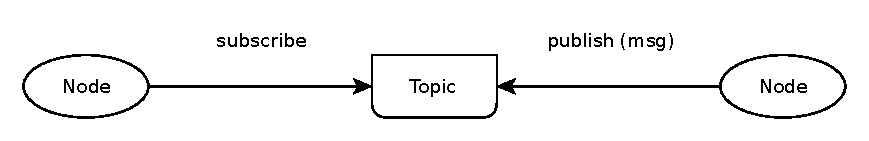
\includegraphics[width=12cm]{kapitel2/ros-topic}
  \caption{Beziehung zwischen Topics und Nodes}
  \label{Kap2:ROSTopic}
\end{figure}

Die zweite Möglichkeit ist die Kommunikation über sogenannte Services. Diese Art der Kommunikation findet nach dem Client-Server-Prinzip statt. Demnach können Nodes, wie in \autoref{Kap2:ROSService} dargestellt, Services anbieten oder diese abfragen. Es handelt sich dabei um eine "`one-to-one"'-Abfrage. Das bedeutet, dass eine Node eine Anfrage an einen Service stellt und nur diese Node antwortet. Das Nachrichtenformat ist das Format "`.srv"'. Definitionen von Services werden in der Regel im Ordner "`/msg"' definiert.

\begin{figure}[t]
  \centering
  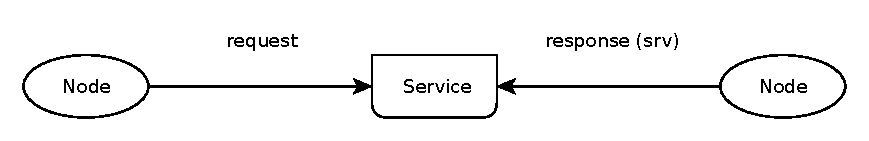
\includegraphics[width=12cm]{kapitel2/ros-service}
  \caption{Beziehung zwischen Services und Nodes}
  \label{Kap2:ROSService}
\end{figure}

Im Allgemeinen beinhaltet jede Nachricht zusätzlich zu den Daten einen sogenannten Header. Dieser enthält eine eindeutige Identifikationsnummer, einen Zeitstempel und eine Frame-ID.

Ein weiterer Bestandteil von \ac{ROS} sind die sogenannten Launch-Files. Diese sollen das Ausführen von mehreren Nodes vereinfachen, da am Ende nur noch ein einziges Launch-File gestartet werden muss. Ein Launch-File wird in XML definiert. Üblich ist es, für alle Launch-Files einen Ordner mit dem Namen "`launch"' zu erstellen. Neben dem Starten von Nodes können Launch-Files auch andere Launch-Files inkludieren. Außerdem kann eine Namensänderung von Topic-Namen definiert werden, um die Kompatibilität zwischen mehreren Packages zu gewährleisten. Dies nennt sich auch Remapping. Zuletzt bieten Launch-Files noch die Option Nodes bei Absturz neu zu starten, die Ausgabe auf dem Bilschirm auszugeben und die Option Konsolenargumente zu verarbeiten.

\lstinputlisting[language=Xml,caption={Beispiel eines Launch-Files in XML},label=lst:LaunchFileXML,float=t]{\srcloc/ROS_Launch-File.xml}

Das Launch-File in \autoref{lst:LaunchFileXML} startet zwei Nodes. Die erste Node veröffentlicht über das \ac{ROS}topic-Node die Message, welche den Befehl zum Motorstart ausführt. Die zweite Node startet die Node, welche Kommandos aufnehmen kann, um den Roboter zu bewegen. Der dritte Block startet ein externes Launch-File, welches wiederum Kommandos für einen Joystick beinhaltet, der Befehle an den p2os\_driver geben kann. Launch-Files sind hilfreich, damit alle Nodes nicht einzeln gestartet werden müssen.

Des Weiteren bietet das System mit den sogenannten Bags die Möglichkeit zum Aufzeichnen und Wiedergeben von Nachrichten bzw. spezifischer Sensordaten. Damit ist es möglich, eine Aufnahme mit der Roboter immer wieder abzuspielen, um einen Fehler zu analysieren, ohne den Roboter erneut durchlaufen lassen zu müssen. Bag-Aufnahmen oder Bag-Wiedergaben können auch in Launch-Files definiert werden. Außerdem lassen sich Aufnahmen sowohl über das Terminal als auch über eine grafische Oberfläche starten und modifizieren, wie in \autoref{Kap2:ROSBag} zu sehen ist.

\begin{figure}[t]
  \centering
  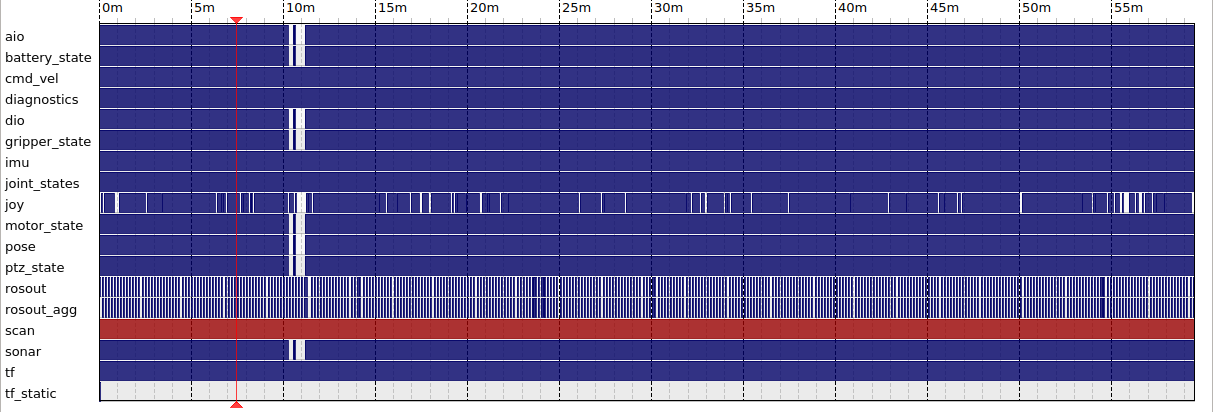
\includegraphics[width=14cm]{kapitel2/rqt-bag}
  \caption{Abspielen eines ROS-Bags mit RQT}
  \label{Kap2:ROSBag}
\end{figure}

Das Robot Operating System bietet zuletzt noch ein mächtiges Kommandozeilen-Tool, mit dem Aufgaben leichter erledigt werden können. Die in \autoref{ROS-Kommandozeile} gezeigten Kommandos, dienen als Überblick über die erläuterten Themen. \autocite{learningROSForRoboticsProgramming} \autocite{gentleIntroductionToROS}
\begin{table}[b]
  \caption{ROS-Kommandozeile}
  \label{ROS-Kommandozeile}
  \renewcommand{\arraystretch}{1.2}
  \centering
  \sffamily
  \begin{footnotesize}
    \begin{tabular}{l l}
    \toprule
    \textbf{Kommando} & \textbf{Erklärung}\\
    \midrule
    \multicolumn{2}{c}{\textit{Allgemein}}\\
    roscore & Startet den ROS-Master\\
    rospack list & Gibt alle Packages aus\\
    roscd package-name & Wechselt das Verzeichnis zu einem Package\\
    rosls & Zeigt die Inhalte eines Packages an\\
    rospack find package-name & Findet das Verzeichnis eines Packages\\
    \multicolumn{2}{l}{}\\
    \multicolumn{2}{c}{\textit{Nodes}}\\
    rosrun package-name exec-name & Startet eine Node eines Packages\\
    rosnode list & Listet alle Nodes auf\\
    rosnode info node-name & Gibt Informationen zu einer Node aus\\
    rosnode kill node-name & Beendet eine Node\\
    \multicolumn{2}{l}{}\\
    \multicolumn{2}{c}{\textit{Topics}}\\
    rostopic list & Listet alle Topics auf\\
    rostopic echo topic-name & Gibt die Inhalte eines Topics aus\\
    rostopic info topic-name & Gibt Informationen zu einem Topic aus\\
    rosmsg show message-type-name & Zeigt den Aufbau der Message an\\
    \multicolumn{2}{l}{}\\
    \multicolumn{2}{c}{\textit{Services}}\\
    rosservice list & Listet alle Services auf\\
    rosservice node service-name & Gibt die Node aus, die den Service anbietet\\
    rosservice info service-name & Gibt Informationen zu einem Service aus\\
    rossrv show service-data-type-name & Zeigt den Aufbau der Service-Message an\\
    \multicolumn{2}{l}{}\\
    \multicolumn{2}{c}{\textit{Launch-Files}}\\
    roslaunch filename & Führt das Launch-File aus\\
    \multicolumn{2}{l}{}\\
    \multicolumn{2}{c}{\textit{Bags}}\\
    rosbag record -a & Zeichnet alle Topics auf\\
    rosbag play filename & Spielt das ROS-Bag wieder ab\\
    rosbag info filename & Gibt Informationen zu einem ROS-Bag aus\\
    \bottomrule
    \end{tabular}
  \end{footnotesize}
  \rmfamily
\end{table}

\section{Pioneer 3-DX}

Im nächsten Schritt wird der zu verwendende Roboter für die Kartierung vorgestellt und dargelegt, wie dieser mit dem Robot Operating System interagiert.

Der Pioneer 3-DX ist ein mobiler Roboter, der in verschiedenen Bereichen der Robotik eingesetzt werden kann, da er beliebig erweiterbar ist. Beispielsweise lässt dieser sich für die Kartierung einsetzen, wenn er um einen Laserscanner erweitert würde. Eine weitere Möglichkeit ist, dass der Roboter alltägliche Aufgaben erfüllen kann, in dem man ihn mit einem Greifarm ausstattet.

Das Modell 3-DX an sich ist 44,5 cm lang, 39,3 cm breit und 23,7 cm hoch, wiegt 9 Kilogramm und kann maximal 25kg tragen. Des Weiteren besteht der Roboter aus zwei Rädern und einem zusätzlichen Stützrad. Die Art des Fahrens ist das sogenannte Differential Drive. Außerdem besitzt der Pioneer 3-DX Ultraschallsensoren sowie Stoßfänger, falls alle anderen Mechanismen zur Verhinderung eines Aufpralls nicht greifen. \autocite{pioneer3operationsmanual}

Für diese Arbeit ist ein Umbau des Pioneer 3-DX eingesetzt worden. Zusätzlich zu den genannten Bauteilen kommt noch ein Computer, ein Laserscanner sowie eine Intertial Measurement Unit (IMU) zum Einsatz. Beim Computer handelt es sich um die Linux Distribution Ubuntu 18.04.2 LTS. Dieser ist auf der Roboter-Basis angebracht. Der Computer hat 4 GB Arbeitsspeicher sowie 2 GB an zusätzlichem SWAP. Der Laserscanner ist der SICK LMS, der ebenfalls auf der Roboter-Basis angebracht ist. Die IMU ist die Tinkerforge Brick 2.0.

\begin{figure}[t]
  \centering
  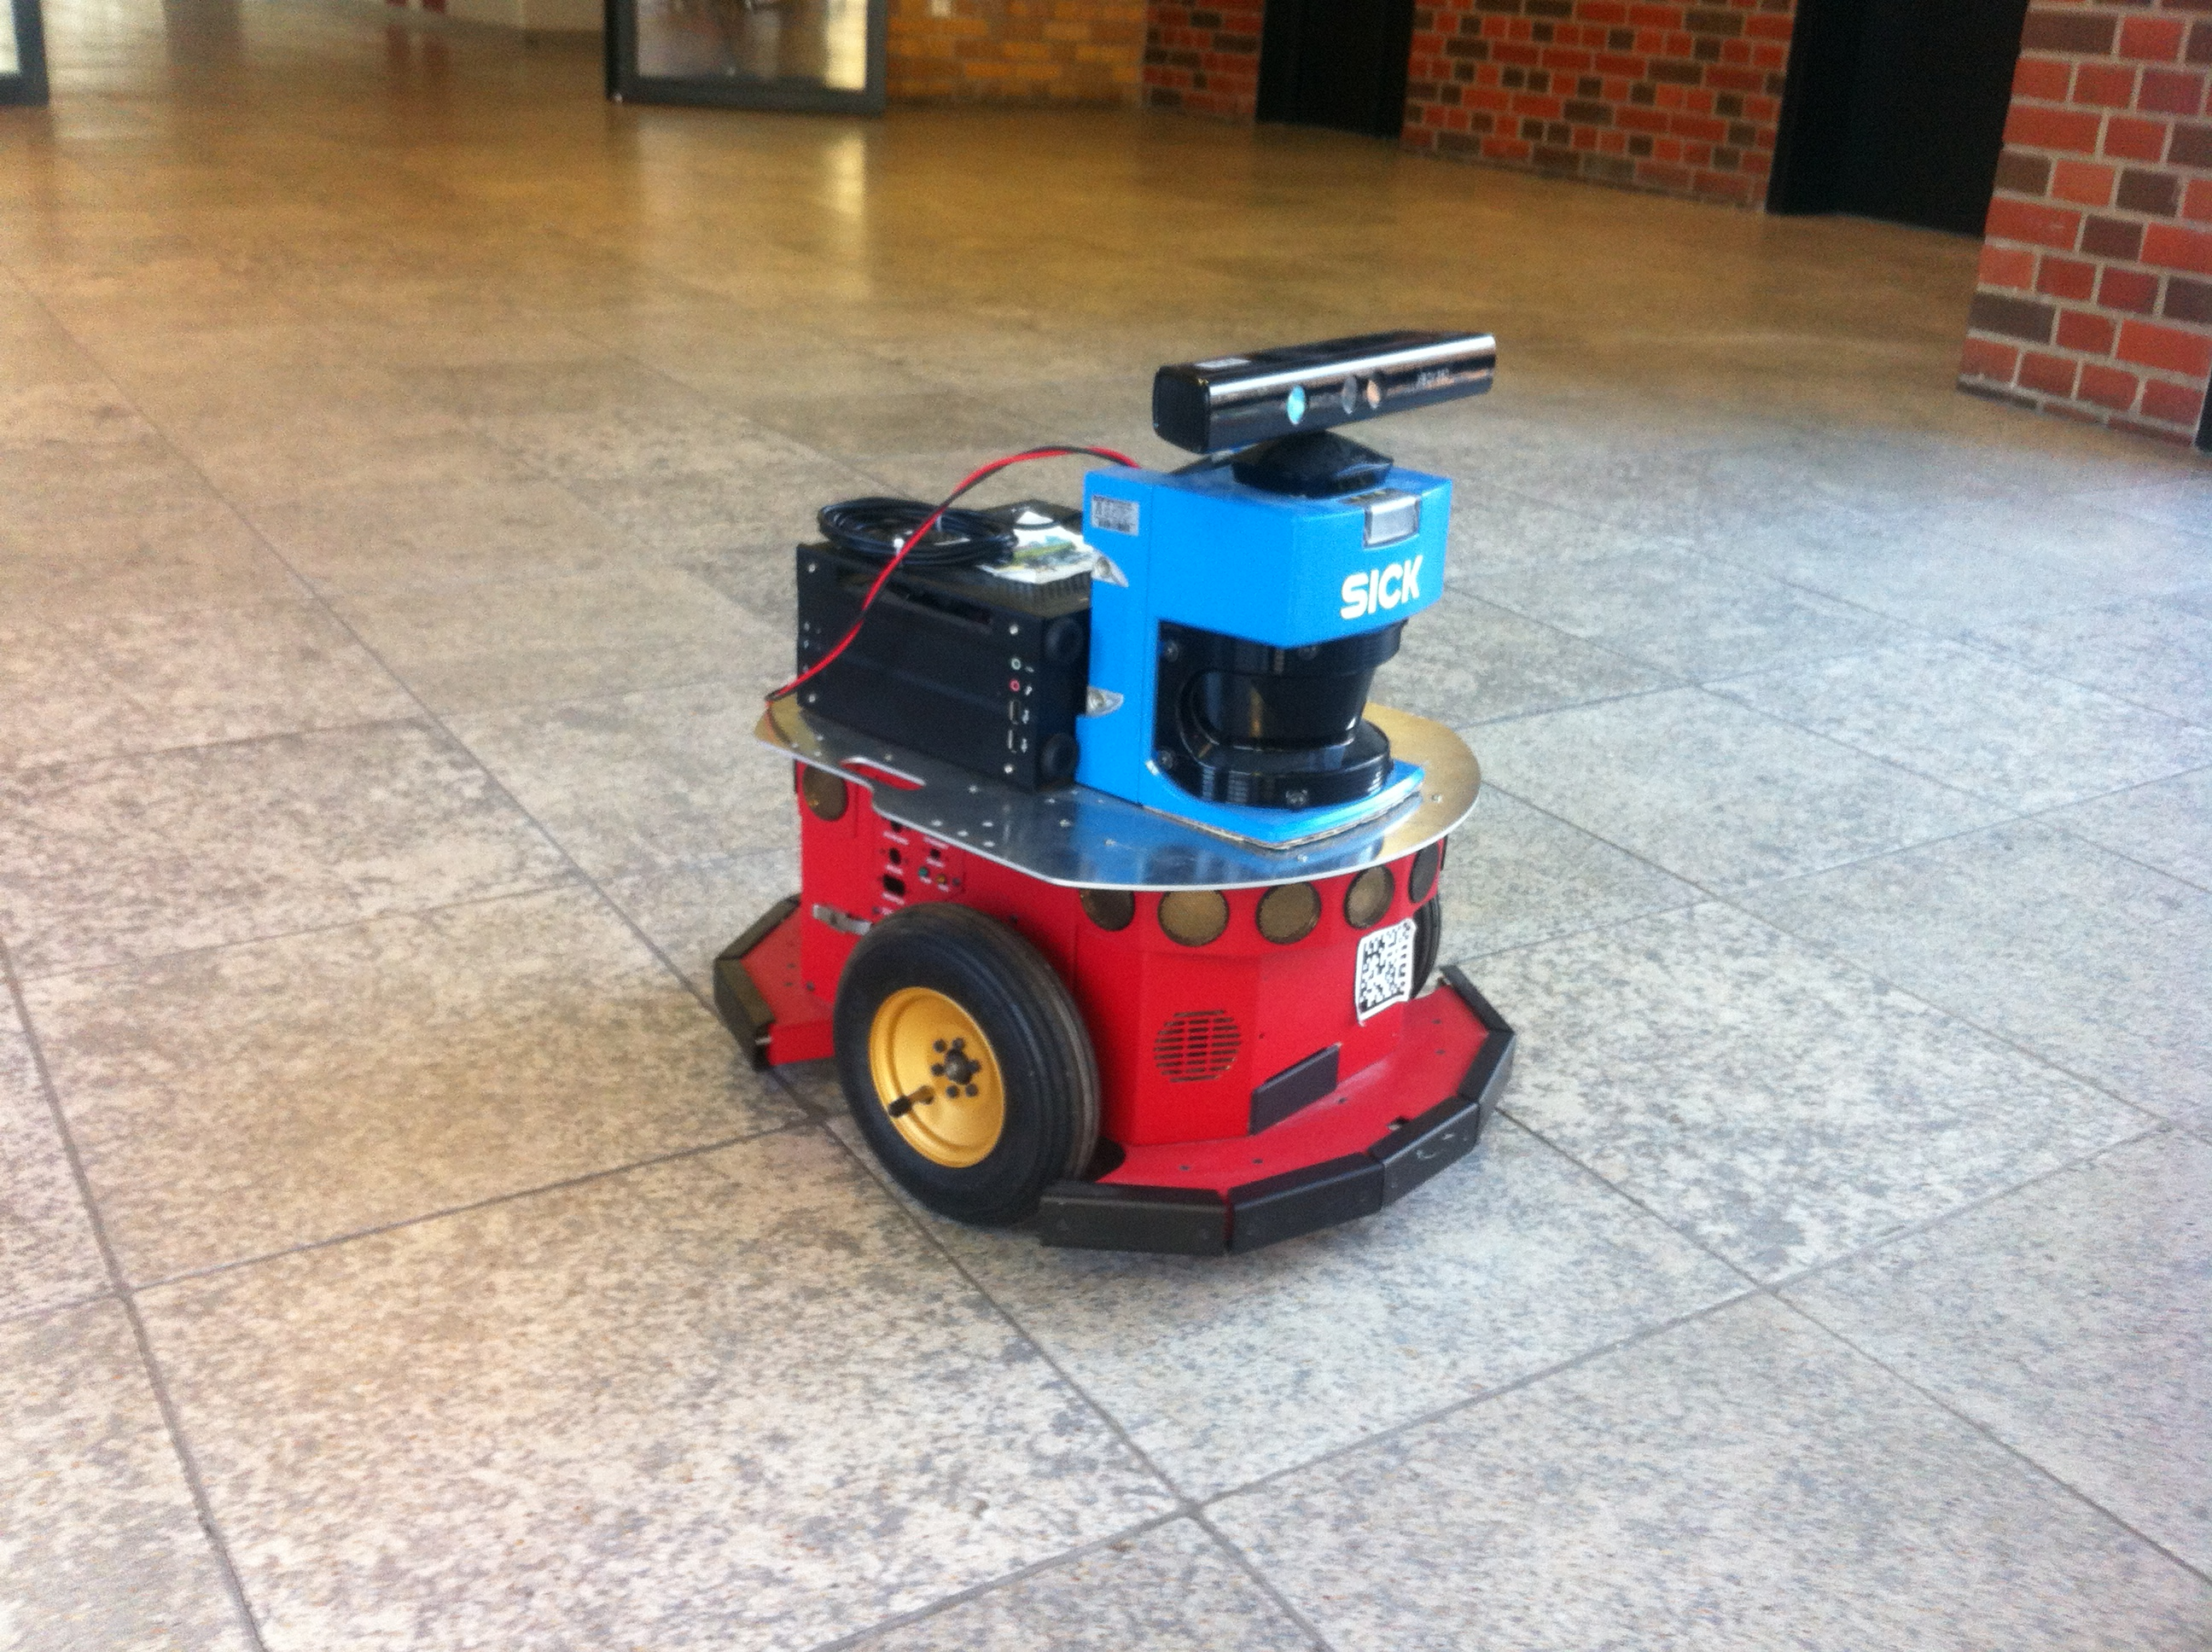
\includegraphics[width=10cm]{kapitel2/pioneer-umbau}
  \caption{Pioneer 3-DX mit Lasercanner, Kinect und Computer}
  \label{Kap2:Pioneer3DX}
\end{figure}

Der Pioneer 3-DX lässt sich im Netzbetrieb oder im Akkubetrieb starten. Dabei sollte mindestens eine Spannung von 12 Volt anliegen. Der Roboter besitzt drei Plätze für Akkus, die gleichzeitig genutzt werden können. \autocite{pioneer3operationsmanual}
\chapter{Kartierungsalgorithmen} \label{Kap3}

In diesem Kapitel wird auf die \ac{ROS}-Packages für die Kartierung eingegangen und deren Unterschiede dargestellt. Dazu wird zunächst immer der Algorithmus und dann das Konzept der Integration in das  \acl{ROS} dargestellt.

Der Anwender sieht während der Algorithmus ausgeführt wird, die Karte, während diese erstellt wird, sofern nicht einfach nur ein Bag-File aufgezeichnet wird. Die Ausgabe ist eine 2D Grid Karte mit jeweils unterschiedlicher Auflösung.

\section{cartographer}

\subsection{Algorithmus}

Der Algorithmus basiert auf einem lokalen und einem globalen Ansatz. Beide Ansätze optimieren die Position der Scans, welche als Formel $ \xi = \left( \xi_{ x }, \xi_{ y }, \xi_{ 0 } \right) $ bestehend aus einer Translation mit $ \xi_{ x } $ und $ \xi_{ y } $ sowie einer Rotation $ \xi_{ 0 } $, definiert sind. Es besteht die Möglichkeit, eine \ac{IMU} zu nutzen, welche hilft, die Scans besser auf die 2D-Welt zu projizieren.

Der lokale Ansatz nimmt die Aufzeichnungen des Laser-Scanners entgegen. Diese werden zu einer sogenannten Submap an der bestmöglichen geschätzten Position hinzugefügt. Eine Submap ist ein Teil der gesamten aufgenommenen Karte. Dieser Prozess wird Scan Matching genannt, und basiert darauf die Lage des Scans zu finden, der die Wahrscheinlichkeitsfunktion der Scanpunkte in der Submap maximiert. Es wird als Lösungsmethode die Methode der nichtlinearen kleinsten Quadrate genutzt.
\begin{align}
    \underset{\xi}{\argmin } { \sum_{k=1}^K {(1 - M_{smooth}(T_{\xi}h_{k}))^{ 2 }} }
\end{align}
$ T_{\xi} $ transformiert $ h_{k} $ vom Scan-Frame zum Sumap-Frame. $ M_{smooth}: R^2 \to R $ bildet die Werte in der lokalen Submap ab. Es wird eine bikubische Interpolation genutzt. Diese sorgt dafür, dass hauptsächlich Werte im Bereich 0 bis 1 vorkommen. Werte außerhalb können auftreten, schaden aber dem Algorithmus nicht.

Das Scan Matching produziert kleine Fehler, die in der Summe große Auswirkungen haben können. Daher besteht das System nicht nur aus einem lokalen Ansatz, welcher auch Frontend genannt wird, sondern auch aus einem globalen Ansatz, der auch Backend genannt wird. Dieser optimiert die lokalen Berechnungen.

Der globale Ansatz wird in regelmäßigen Zeitabständen unabhängig vom lokalen Ansatz durchgeführt. Wenn eine Submap fertig ist, läuft ein sogenanntes Loop Closing ab. Dieser Prozess fügt die einzelnen Submaps zu einer großen Karte zusammen. Dies erfolgt dadurch, dass nahe und passende Scans gesucht werden. Der Algorithmus hinter der Optimerung der Scans und Submaps nennt sich Sparse Pose Adjustment. Es handelt sich dabei wieder um ein Optimierungsproblem. Dieses ist wie folgt definiert:
\begin{align}
    \underset{\Xi^m,\Xi^s}{\argmin } { \sum_{ij} {\rho(\xi_{i}^m,\xi_{j}^s;\Sigma_{ij},\xi_{ij})} }
\end{align}
Dabei wird die Lage der Submaps $ \Xi^m = \left\{\xi_{i}^m\right\}_{i=1,...,m} $, sowie die Lage der Scans $ \Xi^s = \left\{\xi_{j}^s\right\}_{j=1,...,n} $ mit einigen Randbedingungen wie $ \Sigma_{ij} $ und $ \xi_{ij} $ optimiert. Die Verlustfunktion $ \rho $ soll den Einfluss von Ausreißern verringern. 

Insgesamt muss das Loop Closing schneller sein als neue Scans hinzugefügt werden. Durch diesen Prozess werden Loops geschlossen, wenn man einen Ort wiederbesucht. Dazu wird unter anderem ein Branch-and-bound Scan Matching verwendet. \autocite{45466}

\subsection{Verwendung im \acl{ROS}} \label{rosVerwendungCartographer}

Damit der Cartographer eine Karte im \ac{ROS} erstellen kann, müssen zunächst einmal zwei Nodes gestartet werden. Die erste Node ist die Cartographer Node, welche für die simultane Positions- und Kartenerstellung genutzt wird. Dieser Node erwartet eine Liste von Topics, die sie abonniert. (siehe \autoref{Cartographer-Topic-Abonnements}). Der Cartographer publiziert das Ergebnis seiner Berechnungen dann in weiteren Topics (siehe \autoref{Cartographer-Topic-Veröffentlichungen}).

\begin{table}[t]
  \caption{Topic-Abonnements des Packages Cartographer}
  \label{Cartographer-Topic-Abonnements}
  \centering
  \sffamily
  \begin{footnotesize}
    \begin{tabular}{l l l}
    \toprule
    \textbf{Topic} & \textbf{Topic-Typ} & \textbf{Optional}\\
    \midrule
    scan	& sensor\_msgs/LaserScan & Nein\\
    echoes	& sensor\_msgs/MultiEchoLaserScan & Nein\\
    points2	& sensor\_msgs/PointCloud2 & Nein\\
    imu	& sensor\_msgs/Imu & Ja\\
    odom	& nav\_msgs/Odometry & Ja\\
    \bottomrule
    \end{tabular}
  \end{footnotesize}
  \rmfamily
\end{table}

\begin{table}[t]
  \caption{Topic-Veröffentlichungen des Packages Cartographer}
  \label{Cartographer-Topic-Veröffentlichungen}
  \centering
  \sffamily
  \begin{footnotesize}
    \begin{tabular}{l l l}
    \toprule
    \textbf{Topic} & \textbf{Topic-Typ}\\
    \midrule
    scan\_matched\_points2 & sensor\_msgs/PointCloud2\\
    submap\_list & cartographer\_ros\_msgs/SubmapList\\
    \bottomrule
    \end{tabular}
  \end{footnotesize}
  \rmfamily
\end{table}

Die zweite Node ist die Occupancy grid Node, welche die Submaps über das Topic submap\_list verarbeitet und daraus eine Karte erstellt. Das Format in \ac{ROS} ist das nav\_msgs/OccupancyGrid-Format.

Des weiteren benötigt dieser Prozess für jede Sensorkomponente eine Transformation des TF2-Packages. Für jede Komponente sollte entweder ein robot\_state\_publisher oder ein static\_transform\_publisher auf das tracking\_frame sowie das published\_frame, das in der Konfigurationsdatei festgelegt wurde, gesetzt werden. Ein Beispiel dafür ist eine Transformation von der Basis (alias base\_link) zum Laserscanner (alias scan).

Zusätzlich stellt der Cartographer auch Transformationen zur Verfügung. Diese sind je nach Konfiguration die Transformationen von der Karte (alias map) zur Odometrie (alias odom) und zur Basis (alias base\_link). \autocite{cartographerRosWiki}

\section{hector\_mapping}

\subsection{Algorithmus}

Im Gegensatz zum Cartographer basiert der SLAM-Algorithmus hector\_mapping nicht auf der gängigen Konstellation eines Frontends und eines Backends. Das hector\_mapping bietet nur ein Frontend an, welches die typischen Aufgaben ausführt. Dem entsprechend ist der Algorithmus auch nicht für große Karten ausgelegt, bei denen große Loops geschlossen werden müssen. Das Loop-Closing ist nicht explizit implementiert. Besser ist daher die Anwendung in kleinen Karten wie beispielsweise dem RoboCup Rescue, bei dem bestimmte Ziele gerettet werden müssen. Dabei ist die hohe Frequenz des Laserscanners wichtig, damit trotz der Bewegung Ziele auch auf unebenen Ebenen schnell erkannt werden können.

Das hector\_mapping nutzt ausschließlich die Daten des Laser-Scanners als Eingabequelle. Es werden keine zusätzlichen Odometrie-Daten oder IMU-Daten genutzt. Der Prozess besteht aus drei Schritten:
\begin{enumerate}
  \item Preprocessing
  \item Scan Matching
  \item Mapping
\end{enumerate}
Zunächst kommen die Scans im System an und werden zu Point-Clouds weiterverarbeitet, in dem die aktuelle Lage des Roboters und die Daten des Laser-Scanners gemeinsam verarbeitet werden. Es besteht die Möglichkeit, die Liste der Scans vorher zu filtern, um beispielsweise Ausreißer zu entfernen oder um auf Grund der Menge der Datensätze nur einige davon zu betrachten.

Beim Scan Matching werden dann die Scans der Map zugeordnet. Dabei werden beim hector\_mapping die Endpunkte eines Scans mit Hilfe der bisher aufgenommenen Karte optimiert. Dabei kommt das Gauß-Newton-Verfahren inspiriert aus der Computer Vision zum Einsatz. Es wird eine Transformation für den Scan gesucht, die am besten zur aktuellen Karte passt. Es handelt sich wie auch beim Cartographer um ein Minimierungsproblem:

\begin{align}
    \underset{\xi}{\argmin} { \sum_{i=1}^n {[1 - M(S_{i}(\xi))]^{ 2 }} }
\end{align}

Die Funktion $ M $ gibt die Koordinate auf der Karte zurück. Die innere Funktion $ S_{i}(\xi) $ gibt die Koordinaten der Scans. Dieser haben als Parameter die Variable $ \xi $, welche die Lage des Roboters ist.
\begin{align}
    S_{i}(\xi) = \begin{pmatrix}
\cos(\psi) & -\sin(\psi)\\ 
\sin(\psi) & \ \ \ \ \cos(\psi)
\end{pmatrix} \begin{pmatrix}
s_{i,x}\\
s_{i,y}
\end{pmatrix} + \begin{pmatrix}
p_{x}\\
p_{y}
\end{pmatrix}
\end{align}
Das Ziel ist es nun zu berechnen, was passiert, wenn diese 2D-Rotationsmatrix gegen null geht, sprich das globale Minimum zu finden. Des Weiteren wird ein Startwert für $ \xi $ dazu gegeben.

\begin{align}
    \sum_{i=1}^n {[1 - M(S_{i}(\xi + \Delta\xi))]^{ 2 }} \to 0
\end{align}

Jeder Bergsteigeralgorithmus sowie jedes Gradientenabstiegsverfahren kann in einem lokalen Minimum hängen bleiben. Daher wird beim hector\_mapping, um dem entgegenzuwirken, eine Multi-Resolution Map Representation genutzt. \autocite{KohlbrecherMeyerStrykKlingaufFlexibleSlamSystem2011}

\subsection{Verwendung im \acl{ROS}} \label{rosVerwendungHectormapping}

Damit das Package hector\_mapping eine Karte im \ac{ROS} erstellen kann, muss ebenfalls nur eine einzige Node, die hector\_mapping-Node, gestartet werden. Diese benötigt einige Topics (siehe \autoref{hector-mapping-Topic-Abonnements}). Das Ergebnis der Berechnungen publiziert die Node dann in den folgenden Topics (siehe \autoref{hector-mapping-Topic-Veröffentlichungen}).

\begin{table}[t]
  \caption{Topic-Abonnements des Packages hector\_mapping}
  \label{hector-mapping-Topic-Abonnements}
  \centering
  \sffamily
  \begin{footnotesize}
    \begin{tabular}{l l l}
    \toprule
    \textbf{Topic} & \textbf{Topic-Typ} & \textbf{Optional}\\
    \midrule
    scan	& sensor\_msgs/LaserScan & Nein\\
    syscommand & std\_msgs/String & Ja\\
    \bottomrule
    \end{tabular}
  \end{footnotesize}
  \rmfamily
\end{table}

\begin{table}[t]
  \caption{Topic-Veröffentlichungen des Packages hector\_mapping}
  \label{hector-mapping-Topic-Veröffentlichungen}
  \centering
  \sffamily
  \begin{footnotesize}
    \begin{tabular}{l l}
    \toprule
    \textbf{Topic} & \textbf{Topic-Typ}\\
    \midrule
    map\_metadata & nav\_msgs/MapMetaData\\
    map & nav\_msgs/OccupancyGrid\\
    slam\_out\_pose & geometry\_msgs/PoseStamped\\
    poseupdate & geometry\_msgs/PoseWithCovarianceStamped\\
    \bottomrule
    \end{tabular}
  \end{footnotesize}
  \rmfamily
\end{table}

Das hector\_mapping benötigt exakt eine TF-Transformation. Diese ist die Transformation vom Frame, welches zu den eingehenden Scan gehört, zur Basis (alias base\_link).

So wie alle anderen Packages stellt das hector\_mapping ebenfalls eine TF-Transformation zur Verfügung. Dies ist die Transformationen von der Karte (alias map) zur Odometrie (alias odom). \autocite{hectorMappingRosWiki}

\section{gmapping}

\subsection{Algorithmus}

Gmapping ist ein weiterer Kartierungsalgorithmus. Im Gegensatz zum Cartographer und zum hector\_mapping nutzt Gmapping einen Partikelfilter für das \ac{SLAM}-Problem. Dieser ist der Rao Blackwellized Particle Filter.

Dieser Filter basiert darauf die A-posteriori-Wahrscheinlichkeit $ p(x_{1:t} | z_{1:t},u_{0:t}) $ zu berechnen. Dabei ist $ p $ die aktualisierte Wahrscheinlichkeit, ob das Feld auf der Karte gesetzt ist, $ z $ sind die Scans und $ u $ sind die Odometrie-Daten. Dies wird genutzt, um die A-posteriori-Wahrscheinlichkeit über die Karte und die Trajektorie zu berechnen.
\begin{align}
    p(x_{1:t}, m | z_{1:t},u_{0:t}) = p(m | x_{1:t}, z_{1:t})p(x_{1:t} | z_{1:t},u_{0:t})
\end{align}
Dies lässt sich für die A-posteriori-Wahrscheinlichkeit über die Karte $ p(m | x_{1:t}, z_{1:t}) $ berechnen, wenn $ x_{1:t} $ und $ z_{1:t} $ gegeben sind. Um die A-posteriori-Wahrscheinlichkeit für die Trajektorie $ p(x_{1:t} | z_{1:t},u_{0:t}) $ zu berechnen, nutzt der Algorithmus einen weiteren Partikelfilter.

Die Karte wird durch die Scans $ z_{1:t} $, sowie die Trajektorie $ x_{1:t} $ zusammengestellt. Es wird ein Rao-Blackwellized \ac{SIR}-Filter genutzt, der die Scans und die Odometrie-Daten inkrementell zu einer Karte zusammenfügt. Die Odometrie-Daten werden genutzt, sofern sie vorhanden sind. Der Prozess läuft im Allgemeinen wie folgt ab:

\begin{enumerate}
  \item \textit{Sampling}: Über die Verteilung $ \pi(x_{t} | z_{1:t},u_{0:t}) $ werden über die aktuellen Partikel die neuen Partikel entnommen.
  \item \textit{Importance Weighting}: Jeder Partikel erhält eine Gewichtung.
  \item \textit{Resampling}: Partikel mit einer geringen Gewichtung werden durch Partikel mit einer höheren Gewichtung ausgetauscht.
  \item \textit{Map Estimation}: Für jeden Partikel wird die dazugehörige Schätzung auf der Karte berechnet.
\end{enumerate}

Für den gmapping-Algorithmus wird zusätzlich zu dem genannten Ablauf noch eine verbesserte Verteilung berechnet. Außerdem wird ein selektives Resampling genutzt. \autocite{gmapping} \autocite{gmapping2}

\subsection{Verwendung im \acl{ROS}} \label{rosVerwendungGmapping}

Damit das Package gmapping eine Karte im \ac{ROS} erstellen kann, muss nur eine einzige Node, die slam\_gmapping-Node, gestartet werden. Diese benötigt einige Topics (siehe \autoref{gmapping-Topic-Abonnements}). Das Ergebnis der Berechnungen publiziert die Node dann in den folgenden Topics (siehe \autoref{gmapping-Topic-Veröffentlichungen}).

\begin{table}[t]
  \caption{Topic-Abonnements des Packages gmapping}
  \label{gmapping-Topic-Abonnements}
  \centering
  \sffamily
  \begin{footnotesize}
    \begin{tabular}{l l l}
    \toprule
    \textbf{Topic} & \textbf{Topic-Typ} & \textbf{Optional}\\
    \midrule
    scan	& sensor\_msgs/LaserScan & Nein\\
    \bottomrule
    \end{tabular}
  \end{footnotesize}
  \rmfamily
\end{table}

\begin{table}[t]
  \caption{Topic-Veröffentlichungen des Packages gmapping}
  \label{gmapping-Topic-Veröffentlichungen}
  \centering
  \sffamily
  \begin{footnotesize}
    \begin{tabular}{l l}
    \toprule
    \textbf{Topic} & \textbf{Topic-Typ}\\
    \midrule
    map\_metadata & nav\_msgs/MapMetaData\\
    map & nav\_msgs/OccupancyGrid\\
    ~entropy & std\_msgs/Float64)\\
    \bottomrule
    \end{tabular}
  \end{footnotesize}
  \rmfamily
\end{table}

Gmapping benötigt ebenfalls noch einige TF-Transformationen. Dieses ist einmal eine Transformation vom Frame, welches zu den eingehenden Scan gehört, zur Basis (alias base\_link). Des weiteren wird eine Transformation von der Basis (base\_link) zur Odometrie (alias odom) benötigt.

Auch Gmapping stellt eine TF-Transformation zur Verfügung. Dies ist die Transformationen von der Karte (alias map) zur Odometrie (alias odom). \autocite{gmappingRosWiki}
\chapter{Integration der Algorithmen} \label{Kap4}

In diesem Kapitel werden die zuvor beschriebenen Kartierungsalgorithmen in das eigene Package integriert. Dazu werden die Algorithmen als ROS-Packages installiert, durch das eigene Package konfiguriert und mittels eines Launch-Files gestartet.

Das Ziel jeder Integration in das Package ist das Online-\ac{SLAM}, bei dem die Karte während der Aufnahme erstellt wird, als auch das Offline-\ac{SLAM}, bei dem die Karte erst nach der Aufnahme berechnet wird.

\section{Aufsetzen des eigenen Packages}

Um den Roboter nun nutzen zu können, muss dieser mit dem Robot Operating System verbunden werden. Dazu werden einige Packages benötigt, die in einem selbst entwickelten Package zusammengefasst werden.

\begin{itemize}
  \item \textit{p2os:} Dieses Paket stellt die Schnittstelle zur Hardware des Pioneer 3-DX zur Verfügung. Das Package bietet daneben noch die Steuerung mittels Tastatur oder Joystick.
  \item \textit{sicktoolbox\_wrapper:} Dieses Paket startet den Laserscanner Sick LMS und sendet die Scan-Daten an einen Topic.
  \item \textit{ROS-tinkerforge\_sensors:} Dieses Paket startet die Inertial Measurement Unit Tinkerforge Brick 2.0 und sendet die Beschleunigungsdaten an einen Topic.
\end{itemize}

Das eigene Package hat den Namen pioneer3dx\_cartographer und ist in folgende Ordner eingeteilt:

\begin{itemize}
  \item \textit{launch:} Dieser Ordner beinhaltet alle Launch-Files.
  \item \textit{defs:} Dieser Ordner stellt das Xacro-Modell des Pioneers zur Verfügung.
  \item \textit{meshes:} Dieser Order stellt die geometrischen Informationen des Pioneers als STL-Dateien zur Verfügung.
  \item \textit{configuration\_files:} Dieser Order speichert Konfigurationen für den RVIZ oder für Algorithmen.
\end{itemize}

Im ersten Schritt ist im Launch-Ordner die Datei pioneer.launch von Bedeutung, da dieses den Motor, den Laserscanner und die Intertial Measurement Unit des Pioneers, sowie das Xacro-Modell und die benötigten Transformationen startet bzw. lädt. Im weiteren Verlauf des Kapitels wird der Ordner um weitere Launch-Files erweitert, die die einzelnen Kartierungsalgorithmen starten.

Im nächsten Ordner liegt das Modell des Pioneers im Format XML Macros (xacro). Dieses wird zur Laufzeit in das Unified Robot Description Format (URDF) umgewandelt. Ein Modell besteht immer aus mehreren Links und Joints. Ein Link beschreibt einen Teil des Roboters, der Informationen über seine Trägheit und über das Aussehen definiert. Ebenfalls wird in einem Link ein Kollisionsmodell definiert. Links werden über Joints miteinander verbunden. Beispiele für einen Link sind die Räder oder die Basis des Roboters. Das Aussehen eines Links wird über geometrische Informationen im STL-Format definiert. Die STL-Dateien eines jeden Links liegen im Folder meshes. \autocite{xacroRosWiki} \autocite{urdfRosWiki}

Das Modell im xacro-Format lässt sich manuell in das urdf-Format umwandeln. Danach kann eine Grafik der Links und Joints per Kommando erstellt werden.

\lstinputlisting[language=Bash,caption={Umwandlung von xacro in urdf und grafische Darstellung},label=lst:ROSXacro,float=b]{\srcloc/ROS_Xacro-2-URDF.sh}

Für den Pioneer 3-DX ergibt sich dann die folgende Baumansicht in \autoref{Kap2:Pioneer3DXURDF} nach dem Ausführen von \autoref{lst:ROSXacro}.

\begin{figure}[t]
  \centering
  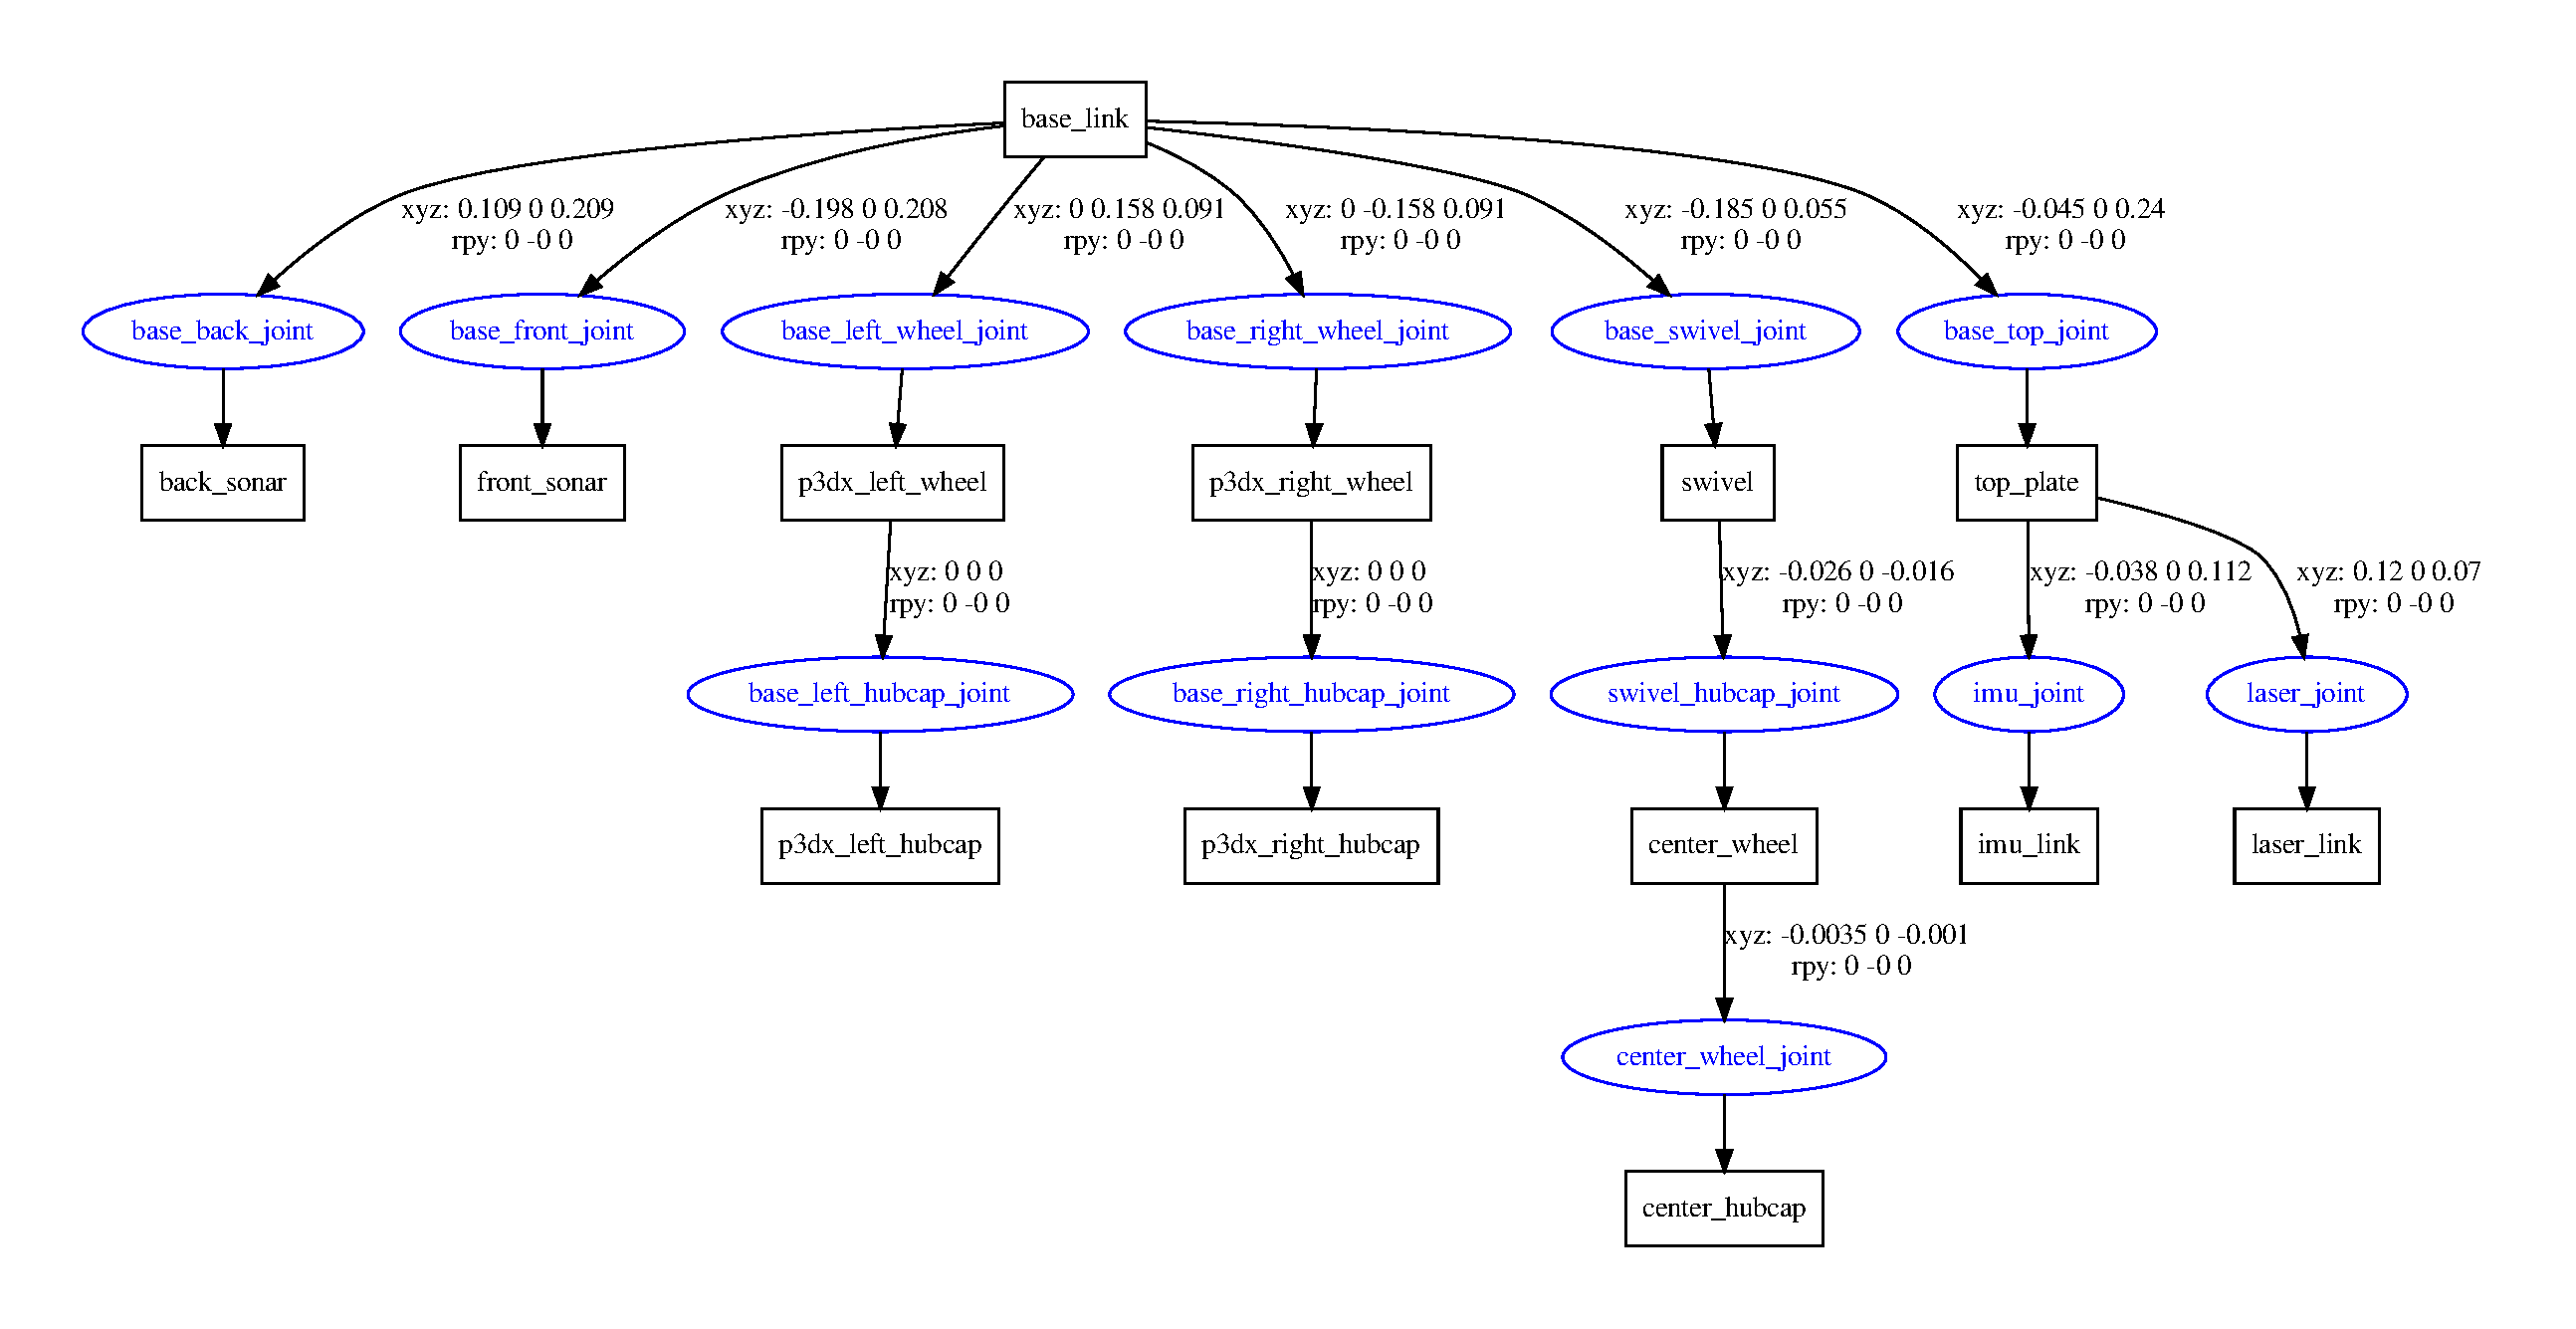
\includegraphics[width=14cm]{kapitel2/pioneer3dx_urdf}
  \caption{Pioneer 3-DX URDF-Modell}
  \label{Kap2:Pioneer3DXURDF}
\end{figure}

\section{Installation der Kartierungsalgorithmen}

Um das eigenen Package um die Kartierungsalgorithmen zu erweitern, müssen die Packages für die Kartierung installiert werden.

\subsection{cartographer}

Für die Installation des Cartographers müssen zunächst einmal die Paketquellen aktualisiert werden. Dann wird das Tool wstool sowie rosdep und Ninja installiert. Danach wird zum Catkin-Workspace gewechselt und einige weitere Installationsschritte mittels dem Tool wstool eingeleitet. Ist dieser Installationsschritt ausgeführt, muss jetzt mittels rosdep noch die Abhängigkeit hinzugefügt werden. Zuletzt muss der Build gestartet werden und der Cartographer installiert werden. Dabei wird das Tool Ninja genutzt, um den Build-Prozess zu verschnellern. \autocite{cartographerInstallation}

\lstinputlisting[language=Bash,caption={Installation des Packages Cartographer},label=lst:ROSCARTOGRAPHERINSTALL,float=t]{\srcloc/cartographer_installation.sh}

\subsection{hector\_mapping}

Die Installation des Packages hector\_mapping gestaltet sich wesentlich einfacher als die des Packages cartographer, da dieses manuell gebaut werden musste. Bei diesem Package wird lediglich der \ac{ROS}-Befehl zur Installation ausgeführt, wie in \autoref{lst:ROSHECTORMAPPINGINSTALL} dargestellt.

\lstinputlisting[language=Bash,caption={Installation des Packages hector\_mapping},label=lst:ROSHECTORMAPPINGINSTALL,float=t]{\srcloc/hector_mapping_installation.sh}

\subsection{gmapping}

Die Installation des Packages gmapping gestaltet sich ebenso einfach wie die des Packages hector\_mapping. Bei diesem Package wird wieder lediglich der \ac{ROS}-Befehl zur Installation ausgeführt, wie in \autoref{lst:ROSGMAPPINGINSTALL} dargestellt.

\lstinputlisting[language=Bash,caption={Installation des Packages gmapping},label=lst:ROSGMAPPINGINSTALL,float=t]{\srcloc/gmapping_installation.sh}


\section{Aufsetzen der Launch-Files und der Konfiguration}

Im nächsten Schritt werden die Launch-Files sowie damit auch die Konfiguration der Kartierungsalgorithmen aufgesetzt. Dabei muss berücksichtigt werden, dass für jeden Algorithmus andere \ac{ROS}-Nodes gestartet und andere Anforderungen an das Transformations-Modul TF erfüllt werden müssen, wie in \autoref{rosVerwendungCartographer},  \autoref{rosVerwendungHectormapping} sowie in \autoref{rosVerwendungGmapping} beschrieben. Pro Algorithmus wird sowohl ein Launch-File für die Online-Kartierung als auch eines für die Offline-Kartierung präsentiert. Bei ersterem wird die Karte während der Aufnahme erstellt. Bei zweiterem wird erst nach der Aufnahme das Bag-File an das Launch-File gegeben und somit wird erst im Nachhinein die Karte erstellt.

Allgemein enthalten alle Launch-Files zusätzlich den Startbefehl für den RVIZ, welcher als Argument eine Konfigurationsdatei enthält. Die Konfigurationsdatei beschreibt die Oberfläche des RVIZ.

\subsection{cartographer}

Der Cartographer definiert für das Online-Kartieren in \autoref{lst:ROSCARTOGRAPHERLAUNCHONLINE} eine Node, welche den Pioneer startet sowie zwei spezifische Nodes für den Cartographer. Die erste Node erhält als Argument eine Konfigurationsdatei, siehe \autoref{lst:ROSCARTOGRAPHERCONFIG}, mit Optionen zum Customizing der Cartographer-Node. Der zweiten Node wird lediglich die Auflösung der resultierenden Karte mitgegeben.

Die Konfigurationsdatei in \autoref{lst:ROSCARTOGRAPHERCONFIG} definiert die genutzten Frames und Nodes, die Frequenz sowie das Sampling von Daten. Dabei waren einige vom Standard abweichende Anpassungen nötig. Wenn eine IMU genutzt werden soll, muss das Attribut TRAJECTORY\_BUILDER\_2D.use\_imu\_data gesetzt werden. Die Anzahl der Laserscanner ist durch das Attribut num\_laser\_scans auf 1 gesetzt. Da 2D-Karten erstellt werden, muss das Attribut publish\_frame\_projected\_to\_2d aktiviert sein.

Das Launch-File für das Offline-Kartieren wird in \autoref{lst:ROSCARTOGRAPHERLAUNCHOFFLINE} gezeigt. Unterschiedlich zu \autoref{lst:ROSCARTOGRAPHERLAUNCHONLINE} ist, dass der Pioneer nicht mehr gestartet werden muss, sondern stattdessen beim Starten an das \ac{ROS}-Bagfile als Argument an das Launch-File übergeben wird, welches beim Start abgespielt wird.

\subsection{hector\_mapping}

Auch beim hector\_mapping in \autoref{lst:ROSHECTORMAPPINGLAUNCHONLINE} wird zunächst die selbe Node wie beim Cartographer definiert, die den Pioneer startet. In den weiteren Zeilen werden einige Konfigurationswerte definiert. Danach wird nur eine Node gestartet, welche diese Werte als Parameter nutzt. Die Konfiguration erfolgt also innerhalb des Launch-Files. In der Konfiguration werden unter anderem die Frames, die Auflösung, Größe und Position der Karte, einige Intervalle sowie der Topic für den Scan definiert.

Das Offline-Kartieren in \autoref{lst:ROSHECTORMAPPINGLAUNCHOFFLINE} erfolgt ähnlich wie das Online-Kartieren. Wie auch beim Cartographer muss das Launch-File des Pioneers nicht mehr gestartet werden. Stattdessen werden wieder die nötigen Nodes für das Einlesen des \ac{ROS}-Bagfiles genutzt.

\subsection{gmapping}

Auch beim gmapping in \autoref{lst:ROSGMAPPINGLAUNCHONLINE} wird zunächst die selbe Node wie beim Cartographer und beim hector\_mapping definiert, die den Pioneer startet. In den weiteren Zeilen werden ebenfalls wie beim hector\_mapping einige Konfigurationswerte definiert. Danach wird nur eine Node gestartet, welches diese Werte als Parameter nutzt. Die Konfiguration erfolgt also wieder innerhalb des Launch-Files. In der Konfiguration wird der Scan-Topic angegeben, sowie Parameter für die Maße und für das Erstellen der Karte.

Das Offline-Kartieren in \autoref{lst:ROSGMAPPINGLAUNCHOFFLINE} erfolgt wieder ähnlich wie das Online-Kartieren. Wie auch bei den anderen Kartierungsalgorithmen muss das Launch-File des Pioneers nicht mehr gestartet werden, sondern stattdessen nur die nötigen Nodes für das Einlesen des \ac{ROS}-Bagfiles.

\section{Starten der Kartierung}

Zum Starten der beschriebenen Online- oder Offline-Kartierungen, werden die gängigen \ac{ROS}-Befehle genutzt. Um diese folgenden Befehle ausführen zu können, muss der Anwender sich im Ordner des \ac{ROS}-Packages befinden.

\subsection{Starten der Online-Kartierung}

Die Online-Kartierung erfolgt immer über einen einzigen roslaunch-Befehl, welcher in \autoref{lst:ONLINE} dargestellt wird.

\lstinputlisting[language=Bash,caption={Online-Kartierung},label=lst:ONLINE,float=t]{\srcloc/online.sh}

\subsection{Starten der Offline-Kartierung}

Bei der Offline-Kartierung muss vorher ein Bag-File mit den gewünschten Topics aufgenommen werden, welches später einem Launch-File als Parameter übergeben wird. Dieses läuft wie in \autoref{lst:OFFLINE} beschrieben ab. Dieses Beispiel nimmt alle verfügbaren Topics auf. Es muss darauf geachtet werden, dass in einem zweiten Terminal das Launch-File des Pioneer vorher gestartet ist, damit Aktionen mit dem Roboter ausgeführt werden können.

\lstinputlisting[language=Bash,caption={Aufnahme eines Bag-Files},label=lst:OFFLINE,float=t]{\srcloc/offline.sh}

Nach der Aufnahme des Bag-Files, kann nun das eigentliche Erstellen der Karte ausgeführt werden. Dies läuft wieder über einen gängigen \ac{ROS}-Launch-Befehl ab, welcher als Parameter den Dateinamen des Bags enthält, wie in \autoref{lst:OFFLINE2} beschrieben.

\lstinputlisting[language=Bash,caption={Offline-Kartierung},label=lst:OFFLINE2,float=b]{\srcloc/offline2.sh}



\lstinputlisting[language=Xml,caption={Online Launch-File für das Package Cartographer},label=lst:ROSCARTOGRAPHERLAUNCHONLINE,float=p]{\srcloc/cartographer_launch_online.xml}

\lstinputlisting[language=Java,caption={Konfigurationsdatei für den Cartographer},label=lst:ROSCARTOGRAPHERCONFIG,float=p]{\srcloc/cartographer_config.lua}

\lstinputlisting[language=Java,caption={Offline Launch-File für das Package Cartographer},label=lst:ROSCARTOGRAPHERLAUNCHOFFLINE,float=p]{\srcloc/cartographer_launch_offline.xml}

\lstinputlisting[language=Xml,caption={Online Launch-File für das Package hector\_mapping},label=lst:ROSHECTORMAPPINGLAUNCHONLINE,float=p]{\srcloc/hector_mapping_launch_online.xml}

\lstinputlisting[language=Xml,caption={Offline Launch-File für das Package hector\_mapping},label=lst:ROSHECTORMAPPINGLAUNCHOFFLINE,float=p]{\srcloc/hector_mapping_launch_offline.xml}

\lstinputlisting[language=Xml,caption={Online Launch-File für das Package gmapping},label=lst:ROSGMAPPINGLAUNCHONLINE,float=p]{\srcloc/gmapping_launch_online.xml}

\lstinputlisting[language=Xml,caption={Offline Launch-File für das Package gmapping},label=lst:ROSGMAPPINGLAUNCHOFFLINE,float=p]{\srcloc/gmapping_launch_offline.xml}

\chapter{Testen der Algorithmen} \label{Kap5}

Im letzten Schritt werden die Kartierungsalgorithmen getestet. Dazu werden verschiedene Szenarien dargestellt. Für jedes Szenario werden Karten durch das Ausführen der Kartierungsalgorithmen erstellt.

Im ersten Szenario wurde aus Tischen ein Rechteck aufgebaut. Ein Tisch ist 1,75m lang. Demnach ist die Breite des Aufbaus 1,75m und die Länge 3,90m, da es auf beiden Seiten noch einen Offset von 20cm gibt. Der Pioneer soll in verschiedenen Arten dort außen herum fahren.

\begin{figure}[t]
  \centering
  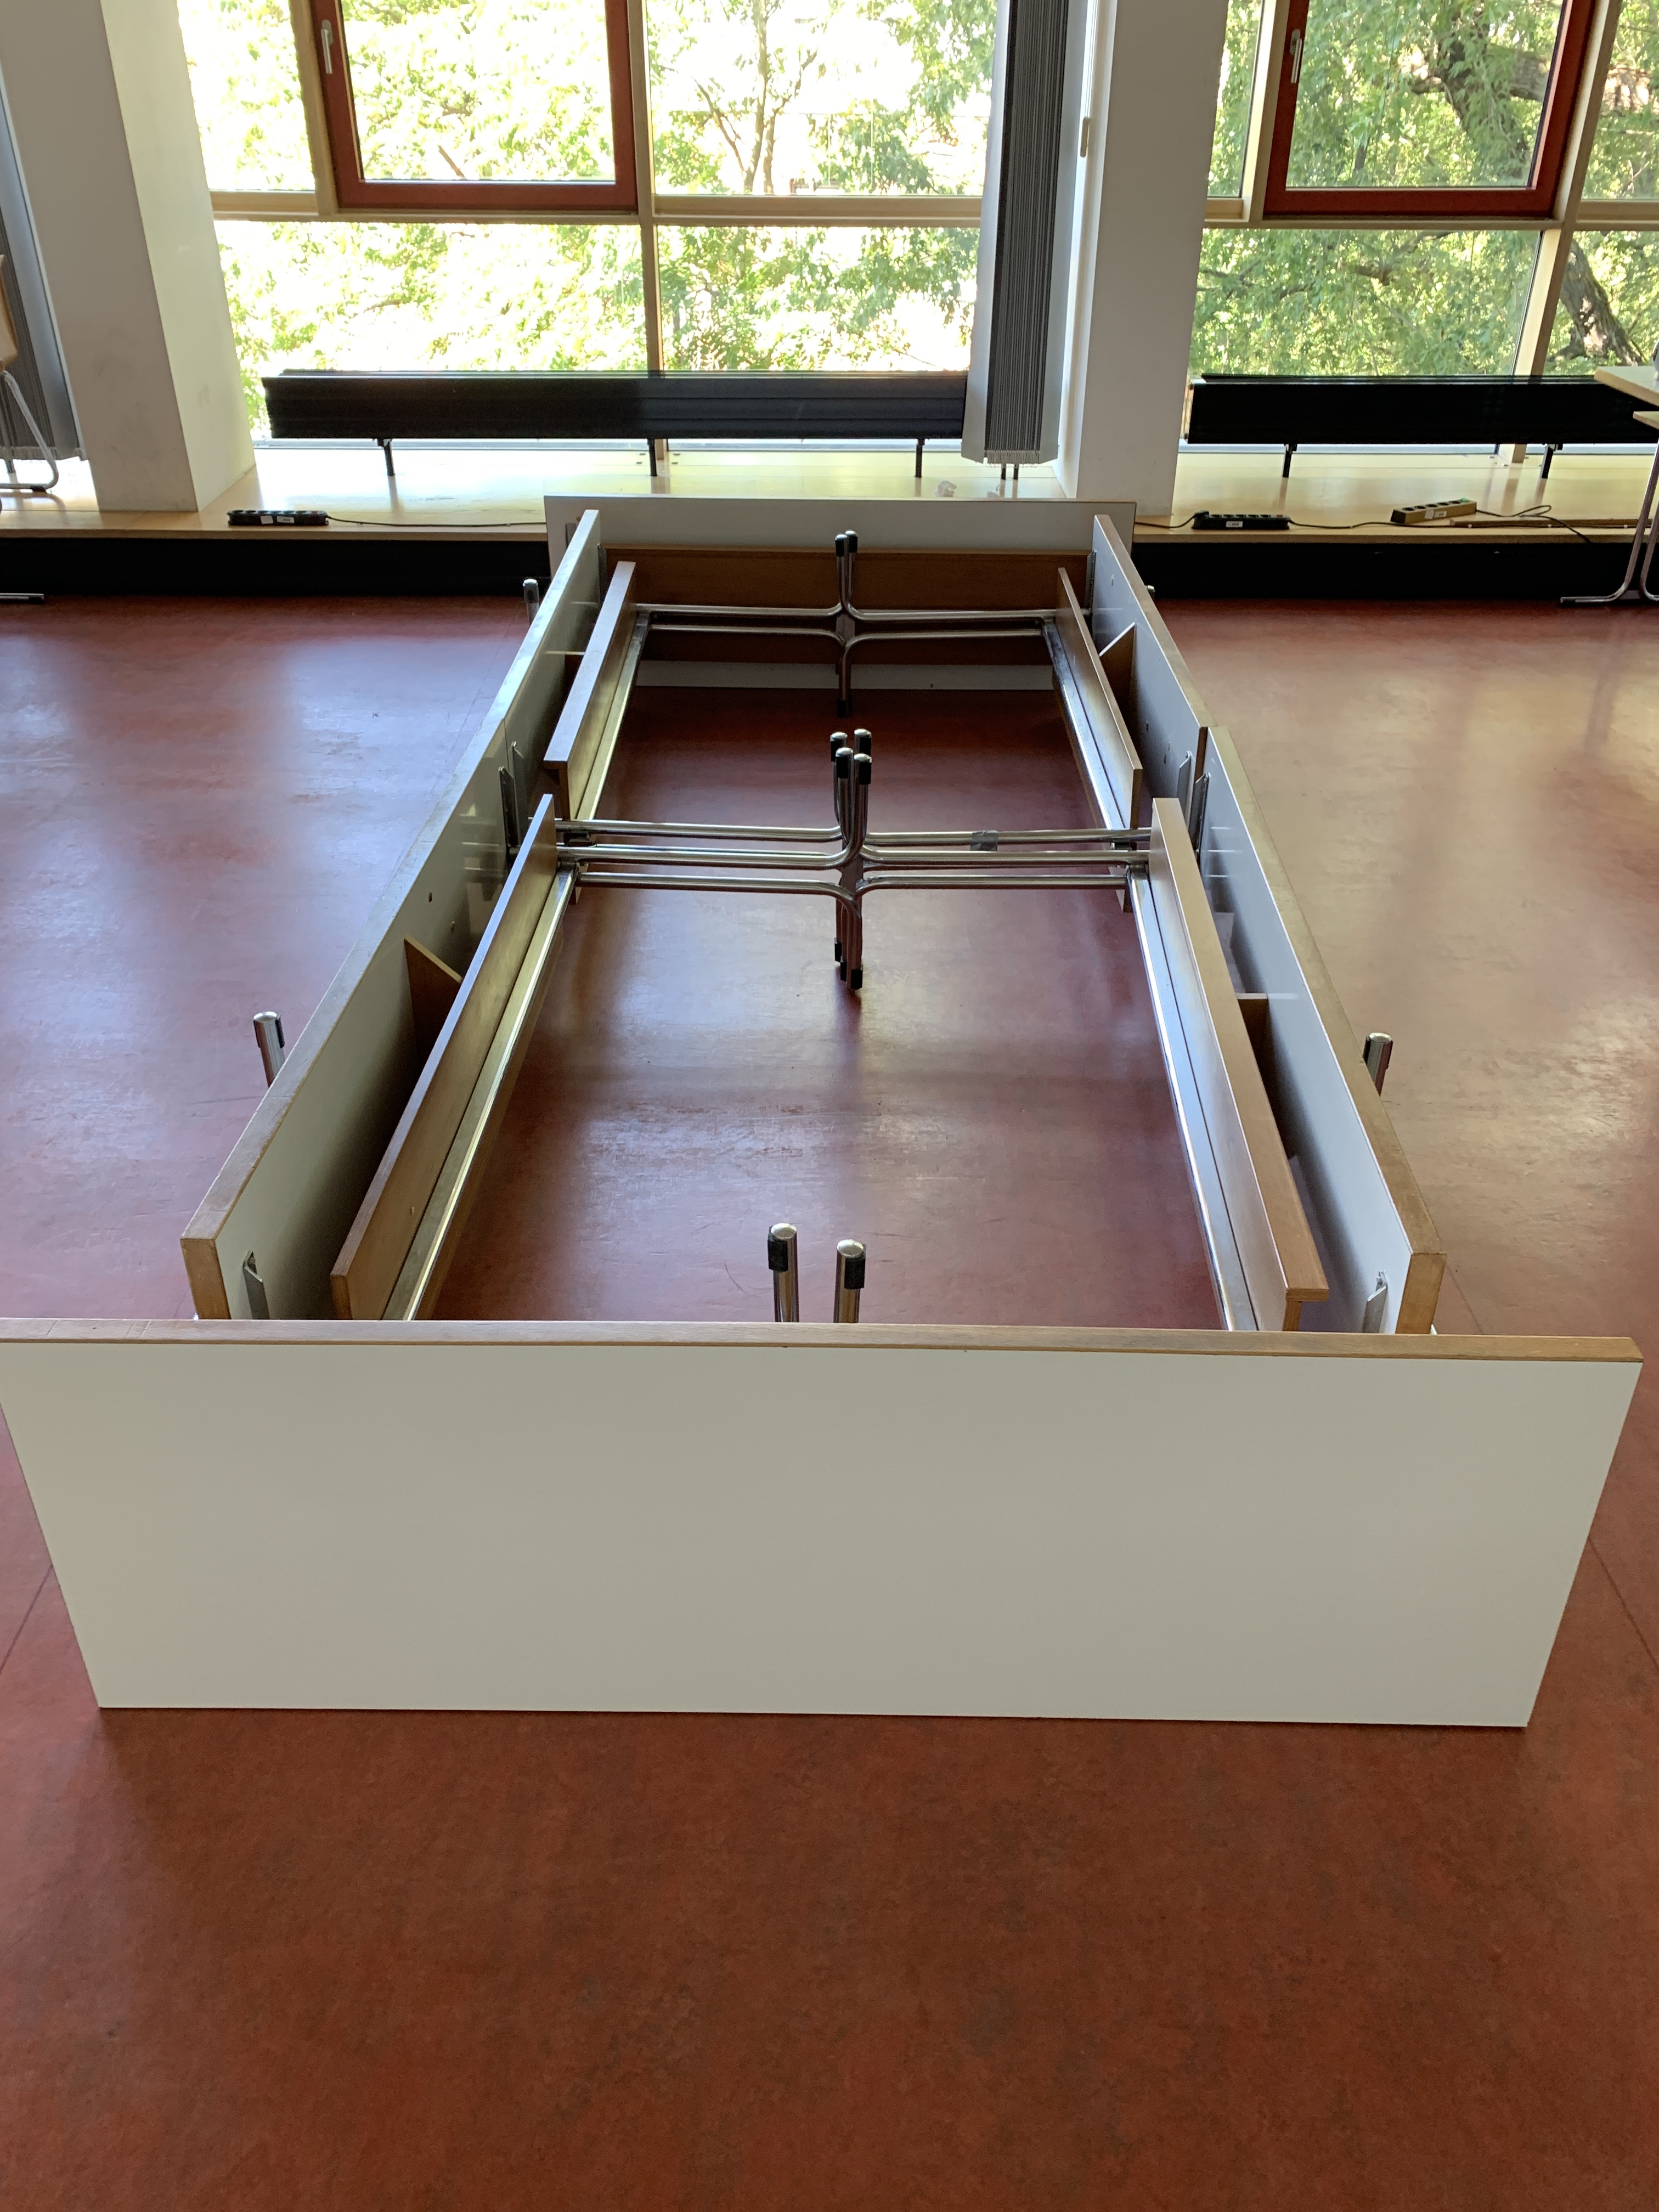
\includegraphics[height=8cm]{kapitel5/testszenario_1}
  \caption{Szenario-Aufbau: Um ein Rechteck fahren}
  \label{Kap5:Szenario1}
\end{figure}

Die erste Aufgabe besteht darin, um das aufgestellte Rechteck zu fahren. Dabei wird möglichst gerade und in einer durchschnittlichen Geschwindigkeit gefahren. Die nächste Aufgabe baut auf der ersten Aufgabe auf. Der Unterschied ist, dass diesmal versucht wird, so schnell wie der Pioneer fahren kann, zu fahren. Die dritte Aufgabe baut ebenfalls auf der ersten Aufgabe auf. Diesmal darf nur rückwärts gefahren werden. In der vierten Aufgabe darf nur in Schlangenlinien gefahren werden.

Im zweiten Szenario soll der Pioneer durch die Vordertür einen Raum betreten und diesen durch die Hintertür wieder verlassen. Das Ziel ist es, auf einer größeren Fläche den Kreis von Scans wieder zu schließen. Die Aufgabe besteht darin, in einer durchschnittlichen Geschwindigkeit durchzufahren und wieder am Endpunkt anzukommen.

Für die Durchführung wird für jede Aufnahme ein Bag-File aufgenommen. Dieses wird beim Auswerten für jeden Algorithmus abgespielt. Dafür dienen die Offline-Launch-Files, welche in \autoref{Kap4} definiert sind.

\section{cartographer}

\begin{figure}[b]
  \centering
  \begin{subfigure}[b]{0.4\linewidth}
    \centering
    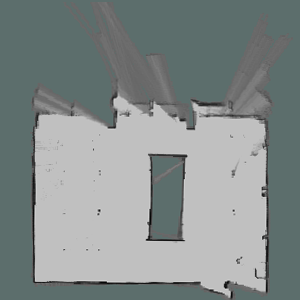
\includegraphics[scale=0.8]{kapitel5/cartographer_umdentisch}
    \subcaption{Normal}\label{kap5:cartographer1}
  \end{subfigure}%
  \qquad
  \begin{subfigure}[b]{.4\linewidth}
    \centering
    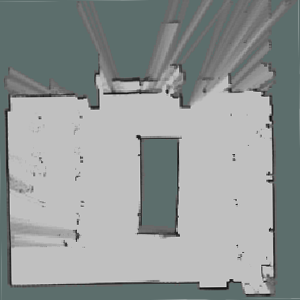
\includegraphics[scale=0.8]{kapitel5/cartographer_umdentischrueckwaerts}
    \subcaption{Rückwärts}\label{kap5:cartographer2}
  \end{subfigure}\\
  \vspace{2\floatsep}
  \begin{subfigure}[b]{.4\linewidth}
    \centering
    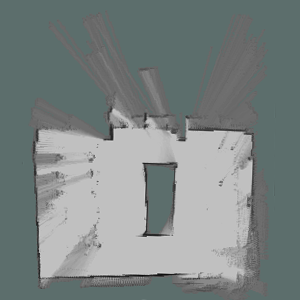
\includegraphics[scale=0.8]{kapitel5/cartographer_umdentischschnell}
    \subcaption{Schnell}\label{kap5:cartographer3}
  \end{subfigure}%
    \qquad
  \begin{subfigure}[b]{.4\linewidth}
    \centering
    
\includegraphics[scale=0.8]{kapitel5/cartographer_umdentischzickzack}
    \subcaption{Schlangenlinien}\label{kap5:cartographer4}
  \end{subfigure}%
  \qquad
  \caption{cartographer: Resultat der Aufnahmen des ersten Szenarios}
  \label{kap5cartographerResultateSzenario1}
\end{figure}

Der Cartographer konnte die Karten zunächst nur ziemlich ungenau zeichnen, da es Probleme mit der Positions- und Drehungsbestimmung des Roboters gab. Der Algorithmus hat diesen Wert falsch geschätzt.

Durch das Aktivieren des \textit{use\_online\_correlative\_scan\_matching} und dem Setzen von \textit{TRAJECTORY\_BUILDER\_2D.ceres\_scan\_matcher.translation\_weight} auf 10
 sowie \textit{TRAJECTORY\_BUILDER\_2D.ceres\_scan\_matcher.rotation\_weight} auf 2 konnten gute Ergebnisse erzielt werden.
 
Das Resultat des ersten Szenarios findet man in \autoref{kap5cartographerResultateSzenario1}. Die Teilabbildung \autoref{kap5:cartographer1} zeigt die normale Auswertung, bei der das Rechteck ziemlich genau dargestellt wird. Auch die Aufgabe in \autoref{kap5:cartographer2}, rückwärts um das Rechteck zu fahren, wird sehr präzise dargestellt. Bei der schnellen Fahrt in \autoref{kap5:cartographer3} ist das Rechteck zu erkennen. Dieses ist allerdings nicht exakt gerade gezeichnet. Gründe dafür könnten sein, dass der Algorithmus zu wenige Daten erhalten hat oder durch die schnellen Bewegungen Ungenauigkeiten in der Odometrie entstanden sind. In \autoref{kap5:cartographer4} wurden Schlangenlinien um das Rechteck gefahren. Dennoch ist das Rechteck gut zu erkennen. Lediglich hat im unteren Teil ein Scan das Rechteck geschnitten. Da dort die Aufnahme geendet hat, hatte der Cartographer keine Zeit mehr, dieses durch weitere Scans zu optimieren. Insgesamt haben alle Auswertungen bis auf die Auswertung \autoref{kap5:cartographer3}, bei der schnell gefahren wurde, den gesamten Umriss des Raums gut erkannt.

\begin{figure}[b]
  \centering
  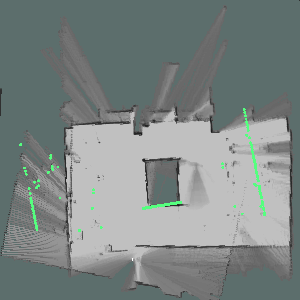
\includegraphics[height=8cm]{kapitel5/cartographer_umdentischmitimu}
  \caption{cartographer: Resultat der Aufnahmen des ersten Szenarios mit IMU}
  \label{kap5cartographerResultateSzenario1a}
\end{figure}

In \autoref{kap5cartographerResultateSzenario1a} wurde eine \ac{IMU} verwendet, um die Auswertung zu verbessern. Dabei gab es Probleme mit der Kalibrierung und der Integration in das eigene \ac{ROS}-Modul, so dass die Auswertung dadurch eher ungenauer wurde. Die \ac{IMU} wurde durch die Konfiguration \textit{TRAJECTORY\_BUILDER\_2D.use\_imu\_data} aktiviert.

Im zweiten Szenario in \autoref{kap5cartographerResultateSzenario2} konnte der Cartographer ohne \ac{IMU} die Scans wieder zusammenfinden und eine ziemlich genaue Karte erstellen.

\begin{figure}[b]
  \centering
  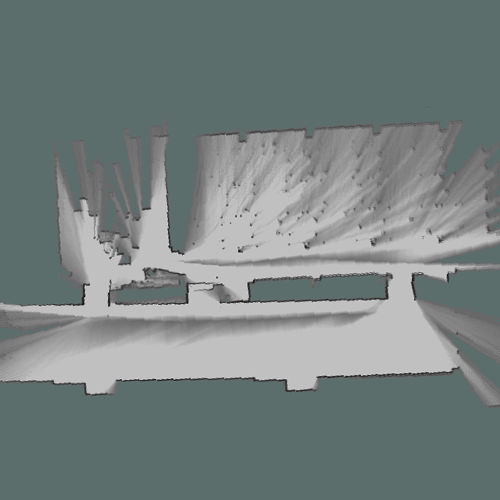
\includegraphics[height=6cm]{kapitel5/cartographer_a207}
  \caption{cartographer: Resultat der Aufnahmen des zweiten Szenarios}
  \label{kap5cartographerResultateSzenario2}
\end{figure}

\section{gmapping}

\begin{figure}[b]
  \centering
  \begin{subfigure}[b]{0.4\linewidth}
    \centering
    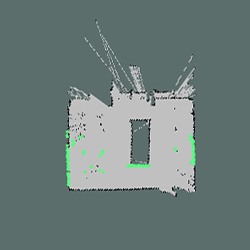
\includegraphics[scale=0.8]{kapitel5/gmapping_umdentisch}
    \subcaption{Normal}\label{kap5:gmapping1}
  \end{subfigure}%
  \qquad
  \begin{subfigure}[b]{.4\linewidth}
    \centering
    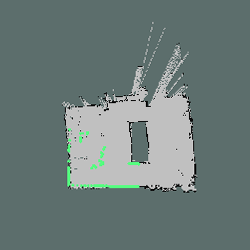
\includegraphics[scale=0.8]{kapitel5/gmapping_umdentischrueckwaerts}
    \subcaption{Rückwärts}\label{kap5:gmapping2}
  \end{subfigure}\\
  \vspace{2\floatsep}
  \begin{subfigure}[b]{.4\linewidth}
    \centering
    
\includegraphics[scale=0.8]{kapitel5/gmapping_umdentischschnell}
    \subcaption{Schnell}\label{kap5:gmapping3}
  \end{subfigure}%
    \qquad
  \begin{subfigure}[b]{.4\linewidth}
    \centering
    
\includegraphics[scale=0.8]{kapitel5/gmapping_umdentischzickzack}
    \subcaption{Schlangenlinien}\label{kap5:gmapping4}
  \end{subfigure}%
  \qquad
  \caption{gmapping: Resultat der Aufnahmen des ersten Szenarios}
  \label{kap5GmappingResultateSzenario1}
\end{figure}

Bei gmapping waren keine Anpassungen nötig, um vernünftige Karten erstellen zu können. In \autoref{kap5GmappingResultateSzenario1} werden die Ergebnisse präsentiert. Die Auswertung \autoref{kap5:gmapping1} ist gut gelungen, da das Rechteck gut erkennbar ist. Beim Rückwärtsfahren in Auswertung \autoref{kap5:gmapping2} ist sowohl der Raum als auch das Rechteck ungenau gezeichnet. Beim Schnellfahren in \autoref{kap5:gmapping3} ist das Rechteck wieder präzise gezeichnet. Es fehlen dort lediglich einige Messwerte, um den Raum auszufüllen. Auch beim Fahren in Schlangenlinien in \autoref{kap5:gmapping4} ist gmapping stabil und produziert ein präzises Resultat. Das gmapping hat außer beim Rückwärtsfahren immer präzise funktioniert.

Auch beim zweiten Szenario in \autoref{kap5GmappingResultateSzenario2} produziert der Algorithmus ein gutes Ergebnis, da die Scans nach dem Zurückkehren guten zusammengefunden wurden.

\begin{figure}[b]
  \centering
  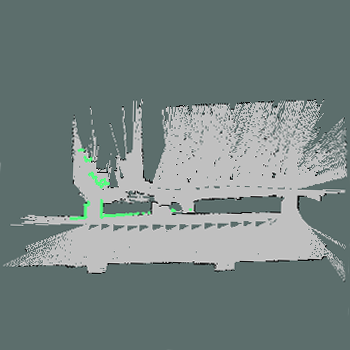
\includegraphics[height=8cm]{kapitel5/gmapping_a207}
  \caption{gmapping: Resultat der Aufnahmen des zweiten Szenarios}
  \label{kap5GmappingResultateSzenario2}
\end{figure}

\section{hector\_mapping}

\begin{figure}[b]
  \centering
  \begin{subfigure}[b]{0.4\linewidth}
    \centering
    
\includegraphics[scale=0.8]{kapitel5/hector_mapping_umdentisch}
    \subcaption{Normal}\label{kap5:hector_mapping1}
  \end{subfigure}%
  \qquad
  \begin{subfigure}[b]{.4\linewidth}
    \centering
    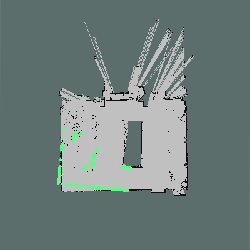
\includegraphics[scale=0.8]{kapitel5/hector_mapping_umdentischrueckwaerts}
    \subcaption{Rückwärts}\label{kap5:hector_mapping2}
  \end{subfigure}\\
  \vspace{2\floatsep}
  \begin{subfigure}[b]{.4\linewidth}
    \centering
    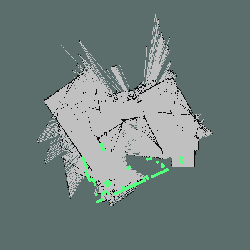
\includegraphics[scale=0.8]{kapitel5/hector_mapping_umdentischschnell}
    \subcaption{Schnell}\label{kap5:hector_mapping3}
  \end{subfigure}%
    \qquad
  \begin{subfigure}[b]{.4\linewidth}
    \centering
    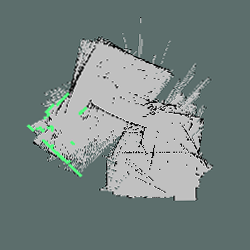
\includegraphics[scale=0.8]{kapitel5/hector_mapping_umdentischzickzack}
    \subcaption{Schlangenlinien}\label{kap5:hector_mapping4}
  \end{subfigure}%
  \qquad
  \caption{hector\_mapping: Resultat der Aufnahmen des ersten Szenarios}
  \label{kap5HectorMappingResultateSzenario1}
\end{figure}

Auch beim hector\_mapping waren keine Anpassungen nötig, um vernünftige Karten erstellen zu können. Die Karte in \autoref{kap5:hector_mapping1} hat wie in den vorherigen Algorithmen ebenfalls gute Ergebnisse erzielt. Beim Rückwärtsfahren in Karte \autoref{kap5:hector_mapping2} ist der linke Teil des Rechtecks verrutscht. Ansonsten ist diese Karte gut gelungen. Kaum gut gelungen sind die Karten, die durch Schnellfahren oder durch Schlangenlinien in \autoref{kap5:hector_mapping3} und \autoref{kap5:hector_mapping4} erzeugt wurden. Bei diesen ist gar kein Rechteck erkennbar und diese sind ziemlich verrutscht. Das hector\_mapping hat hier also nur gut funktioniert, wenn vorwärts oder rückwärts in einer normalen Geschwindigkeit gefahren wurde. Zu viele oder zu schnelle Kurven haben dagegen nicht funktioniert.

Auch im zweiten Szenario in \autoref{kap5HectorMappingResultateSzenario2} haben zu viele Kurven das Ergebnis ungenau gemacht. Der Rest der Karte ist ansonsten präzise.

\begin{figure}[b]
  \centering
  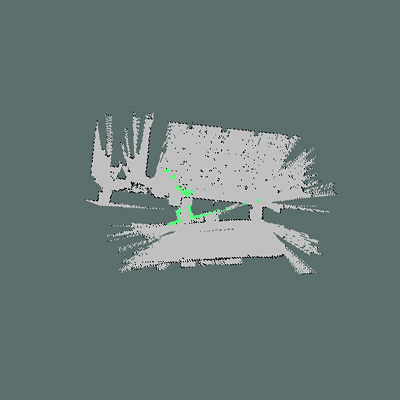
\includegraphics[height=8cm]{kapitel5/hector_mapping_a207}
  \caption{hector\_mapping: Resultat der Aufnahmen des zweiten Szenarios}
  \label{kap5HectorMappingResultateSzenario2}
\end{figure}

\section{Vergleich}

\autoref{tab:vglkartierungsalgorithmen} stellt dar, wie die einzelnen Kartierungsalgorithmen nach einigen Kriterien abgeschlossen haben. 

Zunächst einmal sind die Konfigurationsmöglichkeiten der Algorithmen von Bedeutung. Da bietet der Cartographer eine große Auswahl mit einer guten Dokumentation. Die anderen Algorithmen lassen sich auch konfigurieren, allerdings ist mit dem Cartographer einfach viel mehr möglich, wie zum Beispiel die 3D-Kartierung oder das Verwenden einer \ac{IMU}.

Alle Algorithmen konnten den ersten Test problemlos durchführen. Probleme hingegen gab es beim Rückwärts, Schnell oder Schlangenlinien fahren. Insgesamt schnitt der Cartographer am besten ab, da dieser alle Tests nach einigen Optimierungen der Konfiguration bestanden hat. Der gmapping-Algorithmus hatte Probleme beim Rückwärtsfahren und der hector\_mapping-Algorithmus konnte die Kartierung für eine schnelle Fahrt und eine Fahrt in Schlangenlinien nicht gut durchführen.

Der Test für die \ac{IMU} schlug zwar auf dem Cartographer auf Grund von einer falschen Kalibrierung und einem fehlerhaften \ac{ROS}-Package fehl, dennoch ist es positiv, dass der Algorithmus diese Option als einziger anbietet.

\begin{table}[b]
  \caption{Vergleich der Kartierungsalgorithmen}
  \label{tab:vglkartierungsalgorithmen}
  \centering
  \begin{tabular}{lccc}
    \toprule
    & Cartographer & gmapping & hector\_mapping\\
    \midrule
    Konfigurationsmöglichkeiten	& \harveyBallFull & \harveyBallHalf & \harveyBallHalf \\
    Normal fahren	& \harveyBallFull & \harveyBallFull & \harveyBallFull \\
    Rückwärts fahren	& \harveyBallFull & \harveyBallThreeQuarter & \harveyBallFull\\
    Schnell fahren	& \harveyBallFull & \harveyBallFull & \harveyBallQuarter\\
    Schlangenlinien fahren & \harveyBallFull & \harveyBallFull & \harveyBallQuarter\\
    IMU & \harveyBallQuarter & - & -\\
    \bottomrule
  \end{tabular}
\end{table}
\chapter{Zusammenfassung} \label{Kap6}

Das Ziel der Arbeit war es herauszuarbeiten, welche Kartierungsalgorithmen existieren und wie sich diese für den Pioneer 3-DX Roboter in das \ac{ROS} integrieren, konfigurieren, starten und verbessern lassen.

In \autoref{Kap3} wurden die Funktionsweise sowie die Verwendung im \ac{ROS} der einzelnen Kartierungsalgorithmen vorgestellt.

In \autoref{Kap4} wurden das eigene \ac{ROS}-Package vorgestellt, welches die Launch-Files und Konfigurationen der drei Kartierungsalgorithmen speichert. Außerdem wurde hier dargestellt, wie die Packages installiert werden und wie die Kartierung sowohl online als auch offline gestartet werden kann.

In \autoref{Kap5} wurden dann Tests nach zwei Testszenarien für die Kartierungsalgorithmen Cartographer, gmapping und hector\_mapping durchgeführt sowie ausgewertet. Dabei haben sich gewisse Unterschiede zwischen den Algorithmen herausarbeiten lassen. Es hat sich herausgestellt, dass der Cartographer für die ausgewählten Szenarien auf Grund der Konfigurationsmöglichkeiten und der guten Kartierung am besten abgeschnitten hat.
\chapter{Ausblick} \label{Kap7}

Weiterführend hätte man noch das Thema der 2\nicefrac{1}{2}D-Kartierung aufgreifen können, bei der Elemente wie Treppenabgänge sowie Geländer berücksichtigt werden. Im nächsten Schritt wäre auch eine 3D-Kartierung von Bedeutung, welche es ermöglicht, mehr als ein Stockwerk zu kartieren. Interessant wäre es hierbei mit einem Höhensensor zu messen, in welchem Stockwerk der Roboter sich befindet oder allgemein nicht nur eine 2D-Karte aufzunehmen, sondern durch einen bewegbaren Laserscanner, welcher auch Höhendaten liefern kann, eine Karte zu erstellen. Dafür würde sich beispielsweise der Cartographer gut eignen, da dieser auch einige 3D-Optionen anbietet und grundsätzlich sehr viele Konfigurationsmöglichkeiten hat.

Des weiteren wäre es hilfreich gewesen, die \ac{IMU} vollständig zu kalibrieren und konfigurieren, um zu testen, ob diese den Cartographer-Algorithmus verbessert hätten.

In einem weiterführenden Schritt hätte man noch die Navigation nach dem Erstellen der Karten ausprobieren können. Dabei hätte man vergleichend auf verschiedene Navigationsalgorithmen eingehen können und diese ebenfalls wie die Kartierungsalgorithmen in einem \ac{ROS}-Package bündeln können.
% ------------------------------------------------------------------

\label{lastpage}

% Neue Seite
\cleardoublepage

% Backmatter mit normalem Zeilenabstand setzen
\singlespacing

% Römische Ziffern für die "Back-Matter", fortlaufend mit "Front-Matter"
\pagenumbering{roman}
\setcounter{page}{\value{frontmatterpage}}

% Abkürzungsverzeichnis
\addchap{\hsmaabbreviations}
% Die längste Abkürzung kann in die eckigen Klammern
% bei \begin{acronym} geschrieben, um einen hässlichen
% Umbruch zu verhindern
\begin{acronym}[SLAM]
\acro{SLAM}{Simultaneous Localization and Mapping}
\acro{SIR}{Sampling Importance Resampling}
\acro{IMU}{Inertial Measurement Unit}
\acro{ROS}{Robot Operating System}
\acro{EOL}{End of Life}
\end{acronym}


% Tabellenverzeichnis erzeugen
\cleardoublepage
\phantomsection
\addcontentsline{toc}{chapter}{\hsmalistoftables}
\listoftables

% Abbildungsverzeichnis erzeugen
\cleardoublepage
\phantomsection
\addcontentsline{toc}{chapter}{\hsmalistoffigures}
\listoffigures

% Listingverzeichnis erzeugen. Wenn Sie keine Listings haben,
% entfernen Sie einfach diesen Teil.
\cleardoublepage
\phantomsection
\addcontentsline{toc}{chapter}{\hsmalistings}
\lstlistoflistings

% Literaturverzeichnis erzeugen
\begingroup
\cleardoublepage
\begin{flushleft}
\let\clearpage\relax % Fix für leere Seiten (issue #25)
\printbibliography
\end{flushleft}
\endgroup

% Index ausgeben. Wenn Sie keinen Index haben, entfernen Sie einfach
% diesen Teil.
\cleardoublepage
\phantomsection
\addcontentsline{toc}{chapter}{\hsmaindex}
\printindex

\end{document}
